%===============================================================================
% Autoři: Michal Bidlo, Bohuslav Křena, Jaroslav Dytrych, Petr Veigend a Adam Herout 2018

\chapter{Introduction}
\label{chapter:introduction}


Our~body as same as everything surrounding us emits some radiation. The~dominant wavelengths
belong to the~infrared spectrum and our body senses it as a heat. If we pass its significance
for living creatures and the~fact that the~presence of the~right amount of infrared radiation
is essencial for all the~life as we know it, there is also a~lot of usage in the~industry or
generally -- technology.

Infrared waves are used in various devices. From nightvision devices, astronomical telescopes to personal
electronics (infraport, TV remote controller). This thesis focuses on the usage in PIR
sensors -- electronic devices that changes its output based on the amount of received infrared
radiation.

The PIR sensors are used around us a lot even though we might not know it. We all know the waving
of hands towards the~sensor in a~hallway so the light would turn on and we could tie our shoes,
or the~self-opening door in shopping malls or self-rotating door in banks. These mechanisms mostly
use PIR sensors.

\begin{figure}[h!]
  \begin{center}
    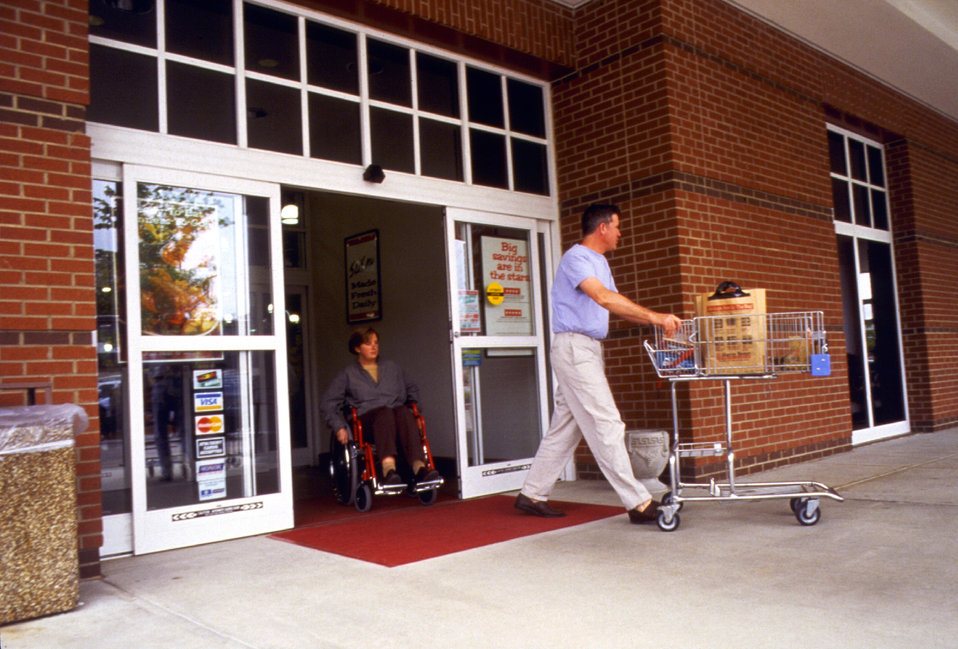
\includegraphics[width=0.5\textwidth]{img/automaticdoorway.jpg}
    \caption{PIR sensor: automatic doorway. \cite{automaticdoorway} \label{fig:automaticdoorway}}
  \end{center}
\end{figure}

PIR sensors offer even more than stating a presence of person. It is possible to~process sensor
output signal to~get more information about~sensed space - a~position of~person, a~number of~people.
Especially when more sensors are used.

The localization using PIR is still matter of intense research, a number of articles has been
written on it. This thesis suggests multisensor attitude and a usage of fuzzy logic to merge
sensor's outputs.



%\chapter{Abstract}
%\label{abstract}
%10 lines 
%Description of problem
%Solution and focus
%Maybe brief conclusion and application







\chapter{State of the art}
\label{theory}


\section{Physics of radiation}

In the~modelled system equations calculating with~infrared radiation are being used -- to~understand
them properly it is necessary to describe what is a~radiation, where does it come from and how can
we measure it. 

As it was already mentioned in the~chapter \ref{chapter:introduction}, every object whose temperature
is higher than absolute zero emits an~electromagnetic radiation.
\begin{equation}
T_{obj}>0~K\equiv -273.15^{\circ}C
\end{equation}
It is caused by a~charged subatomical particles (electrons, protons) that are undergoing an~acceleration,
emitting an~energy in a~form of photon -- electromagnetic radiation.


\subsection*{Characteristics}
The~electromagnetic radiation have a~number of measurable characteristics. The~most significant ones
are {\it frequency} $f$ and {\it wavelength} $\lambda$. Due to the~constant speed of the radiation $v$
aka speed of light $c = v = 3\cdot10^{8}~m\cdot s^{-1}$ not dependent on the frequency, they are
propotional and mutually transferrable.
\begin{equation}
f=\frac{v}{\lambda}=\frac{c}{\lambda}=\frac{3\cdot10^{8}}{\lambda}
\end{equation}

Electromagnetic waves are being divided into categories according to their usage by the wavelength
$\lambda$. With increasing wavelength~$\lambda$ it is gamma, X-rays, ultraviolet (UV), visible light,
infrared (IR) and radio waves. This is called electromagnetic spectrum and it is shown in the image
\ref{fig:spectrum}.

\begin{figure}
\begin{center}
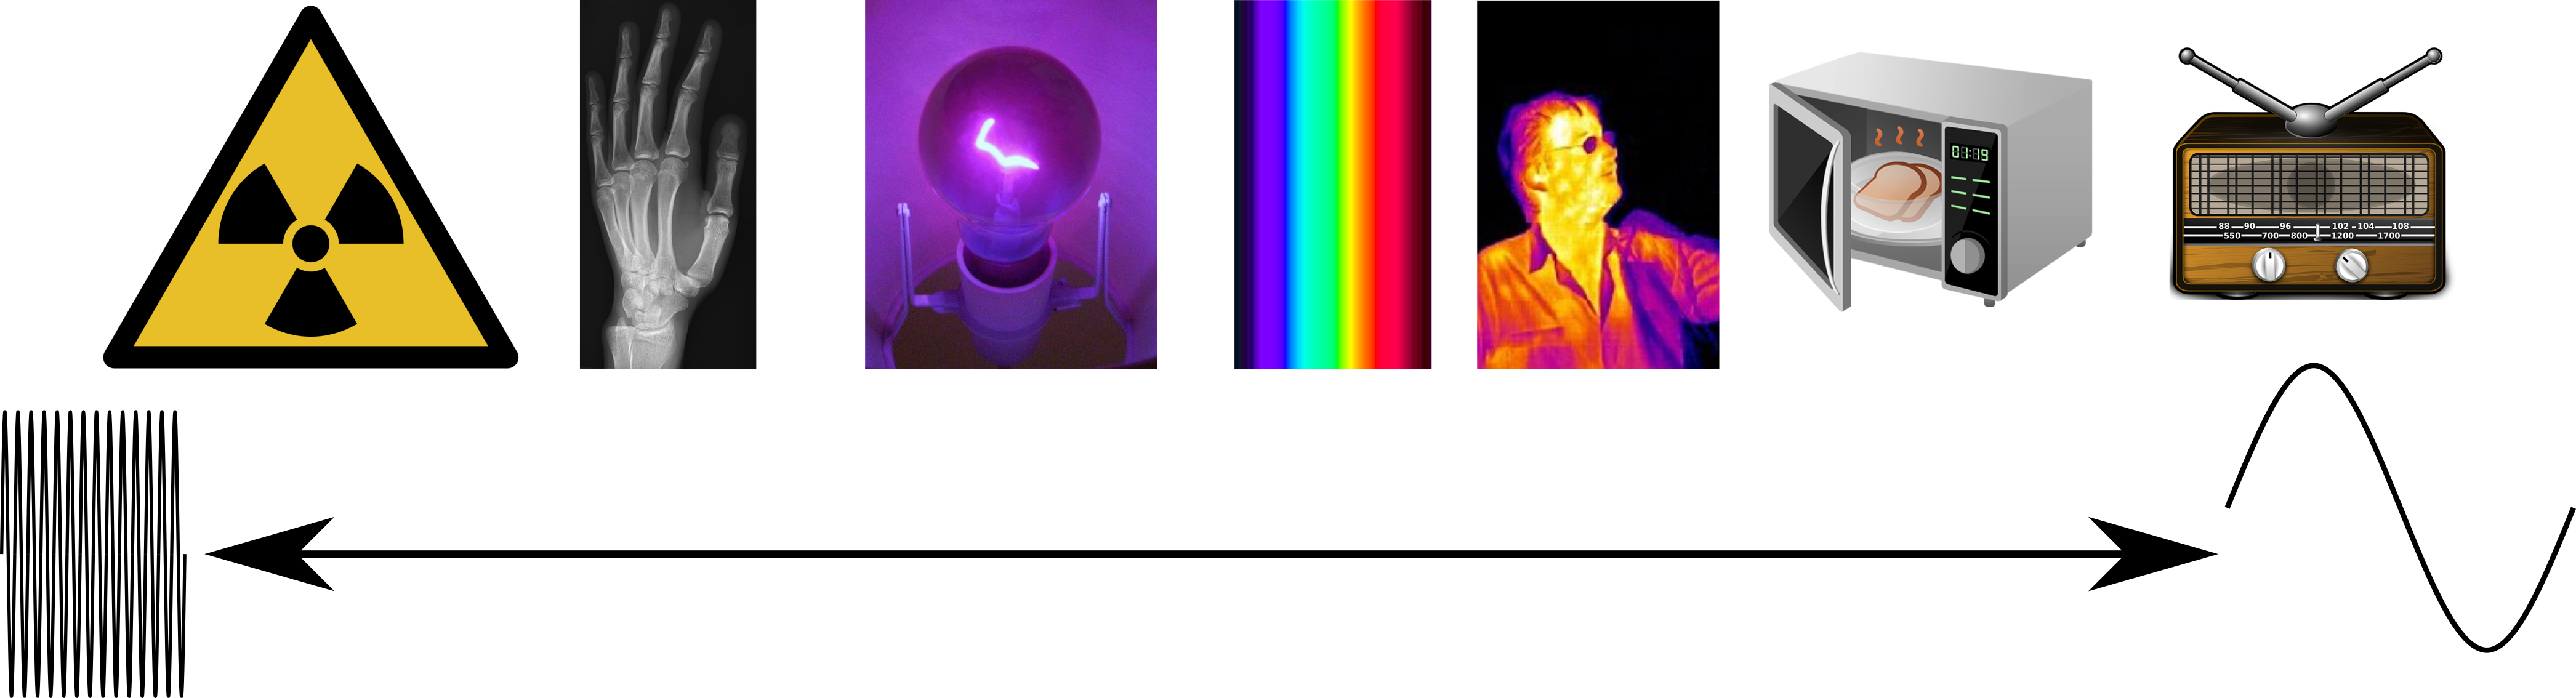
\includegraphics[width=0.8\textwidth]{img/spectrum.png}
\caption{Electromagnetic spectrum.\label{fig:spectrum}}
\end{center}    
\end{figure}

Another measurable characteristic is an~energy of the~radiation $Q$,$E$ or $W$. It is linearly dependend
on its frequency $f$ and can be computed using Planck constant $h=6.63\cdot10^{-34}~J\cdot s $.
\cite{NasaEMSpectrum}
\begin{equation}
W = h\cdot f
\end{equation}

The~power of the~radiation $\Phi$ is called {\it radiant power} or rather {\it radiant flux}. As a~regular
power it is energy per time, since the radiation is four-dimentional, partial derivations must be used.
\begin{equation}
\Phi = \frac{\partial W}{\partial t}
\end{equation}

The radiant power per unit surface is a~flux density. It is called either {\it radiant exitance} $M$
when emitting or {\it irradiance} $E$ when receiving.
\begin{subequations}
\begin{equation}
M = \frac{\partial \Phi_{emitted}}{\partial S_{sender}}
\end{equation}
\begin{equation}
E = \frac{\partial \Phi_{received}}{\partial S_{receiver}}
\end{equation}
\end{subequations}
The~Stefan-Boltzmann law defines irradiance of electromagnetic radiation as
\begin{equation}
I = \sigma \cdot T^4
\end{equation}
where $\sigma = 5.6704\cdot 10^{-8} Wm^{-2}K^{-4}$ is the~Stefan-Boltzmann constant and $T$ is a~thermodynamic
temperature.

Power per unit solid angle $I$ is called {\it radiant intensity}. With dividing by an~area of the~item
projected from certain direction we get an~amount of power emitted in that~direction called {\it radiance} $L$.
\begin{subequations}
\begin{equation}
I = \frac{\partial \Phi}{\partial \Omega}
\end{equation}
\begin{equation}
L = \frac{\partial I}{\partial S cos(\theta)}
\end{equation}
\end{subequations}
Other characteristics of radiation can be seen in the~table \ref{table:units}. \cite{iso800007} \cite{TemperatureMeasuring}

\begin{table}
\begin{tabular}{|c|c|c|l|} \hline
\textbf{Name}             & \textbf{Symbol} & \textbf{Unit}                 & \textbf{Definition}                             \\ \hline
Radiant flux        & $\Phi$          & $W$                           & Power transfered by a radiation.                \\ \hline
Radiant exitance    & $M$             & $W\cdot m^{-2}$               & Sent $W$ per sender's surface.                  \\ \hline 
Irradiance          & $E$             & $W\cdot m^{-2}$               & Received $W$ per receiver's surface.            \\ \hline
Radiant intensity   & $I$             & $W\cdot sr^{-1}$              & $W$ per unit solid angle.                       \\ \hline
Radiance            & $L$             & $W\cdot sr^{-1}\cdot m^{-2}$  & $I$ per sender's area projected to a direction. \\ \hline
\end{tabular}
\caption{Radiation characteristics.\label{table:units} \cite{TemperatureMeasuring}}
\end{table}



\newpage
\section{Temperature homeostasis}
The animal bodies require physical and chemical conditions in order to work properly (or at all). One of
the physical aspects is a temperature. There are generally three types of animals -- {\it ectotherms},
{\it endotherms} and {\it mesotherms}.

Ectotherms do not regulate its body temperature and rely on an external source, endotherms keeps it
constant independently on the environment, so called {\it homeothermy}\footnote{Homeothermy is an aspect
of homeostasis. It means keeping its inner body temperature within the preset limits.}. Mesotherm
strategy is then something in between.

Endotherm groups are birds and mammals, the most significant ectotherm group are reptiles. They compensate
it with basking in the sun. The thermal characteristics of these groups can be seen in the figure \ref{fig:thermoregulatory}.

\begin{figure}[h!]
\begin{center}
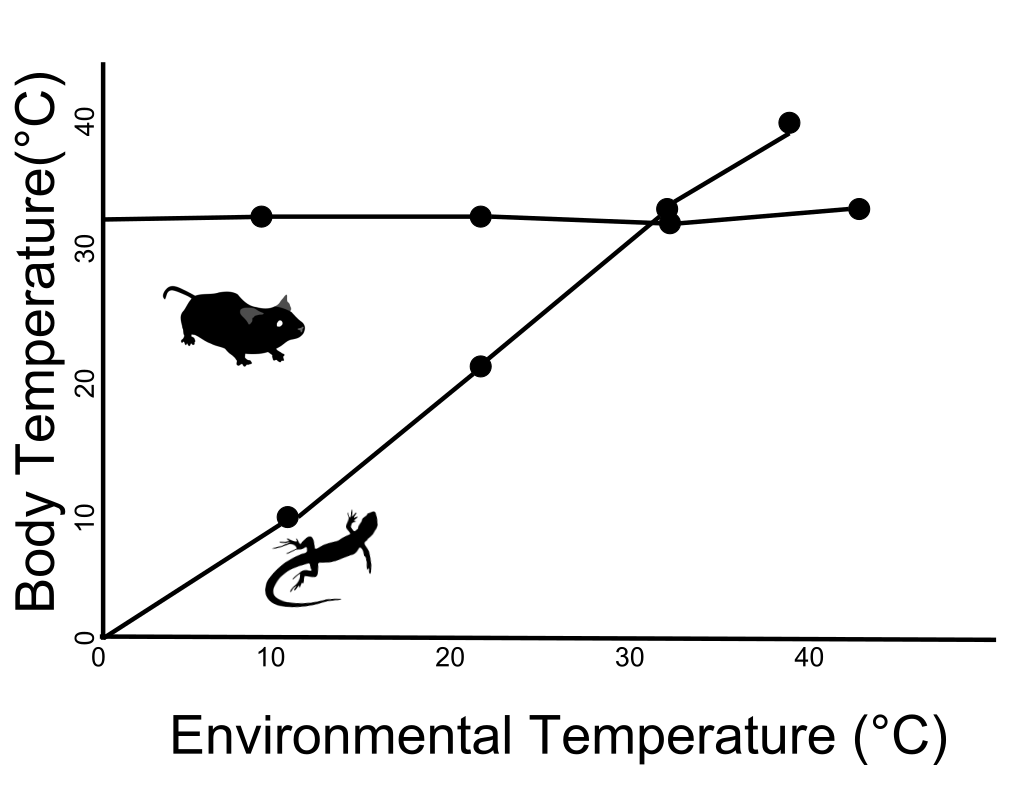
\includegraphics[width=0.4\textwidth]{img/thermoregulatory.png}
\caption{Thermal regulation graph.\label{fig:thermoregulatory}\cite{thermoregulatory}}
\end{center}    
\end{figure}

Human body temperature $T_{HB}$ varies in $\langle 36^{\circ}C; 38^{\circ}C \rangle$, in the hyperthermia
it can rise up to $40^{\circ}C$. The figure \ref{fig:bodywavelength} shows the radiation wavelength composition.
The peak wavelength (temperature $37^{\circ}C$ or $310.15~K$) can be calculated with the Wien's displacement law.
\begin{equation}
\lambda_{max}=\frac{b}{T}=\frac{2.8977729 \cdot 10^{-3}}{310.15} = 9.3431~\mu m
\end{equation}

\begin{figure}[h!]
\begin{center}
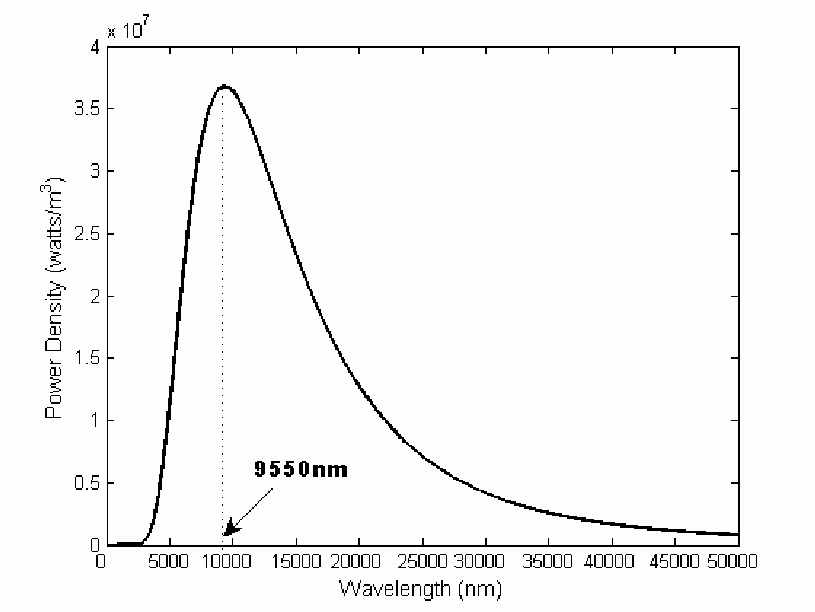
\includegraphics[width=0.4\textwidth]{img/bodyradiation.png}
\caption{Human body radiation wavelength.\cite{BodyRadiation}\label{fig:bodywavelength}}
\end{center}    
\end{figure}





\newpage
\section{Radiation perception}

\subsection*{Radiation processed by organisms}
This~thesis describes a~particular way how to use the~infrared radiation. Very important beginning of such
work is always studying existing applications. Unforgettable one is a~nature -- how evolution enabled 
various organisms to~use it.

Many animals can process parts of electromagnetic spectrum. Eyes enables mammals, cephalopods and arthropods
to sense a visible light, some insects can even see a~part of UV. Additionally organisms including human often
have thermoreceptors in~their skin so they can get information about intensity of infrared radiation around them.


\paragraph{Visible light}
\label{subsection:eye}
PIR~sensor structure is obviously inspired by a~human eye. Human eyes can process radiation
$\lambda \in \langle 380~nm;760~nm \rangle$ called visible light, one of the~bands of an~electromagnetic spectrum.
Seeing means receiving a light from a~light source reflected by the~surface of an~observed object to our retina.
A~biological system composed of~light-sensitive cells {\it rods} and {\it cones} propagates the~information
through nerves to brain.

A~ray coming to an~eye is going through a~converging lens, which changes its~trajectory aiming to~the~retina,
in~the~best case to~the~most sensitive place with a~lot~of~the~rods and cons called {\it Fovea~centralis}.
\cite{LightEyeVision}

\begin{figure}[h!]
\begin{center}
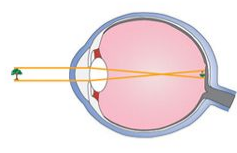
\includegraphics[width=0.3\textwidth]{img/eye.png}
\caption{Structure of an eye. \cite{Eye}\label{fig:eye}}
\end{center}    
\end{figure}


\paragraph{Heat}
The~infrared rays surrounds us during our whole life, we sense it as~heat. The~heat receptors called
{\it thermoreceptors} in our body are located on its~surface (in the~skin), but also in~organs.
The~structure of~a~skin is shown in the figure \ref{fig:skin}. 

There is a~difference between sensing a~visible light and an~infrared radiation. Visible light comes
mostly reflected from the surface, while the IR can originate only from the~primary source -- warm item.

Our skin contains two types of~thermoreceptors: sensing cold, colder than a~body temperature and
hot, hotter than a~body temperature. The~skin structure is shown in~the~figure \ref{fig:skin}.
This is already well described, on the~other hand the~evaluation center of~these receptors in~the~brain
and its~mechanisms is~not fully understanded yet and a~matter of current research. \cite{BodilySenses}

\begin{figure}[h!]
\begin{center}
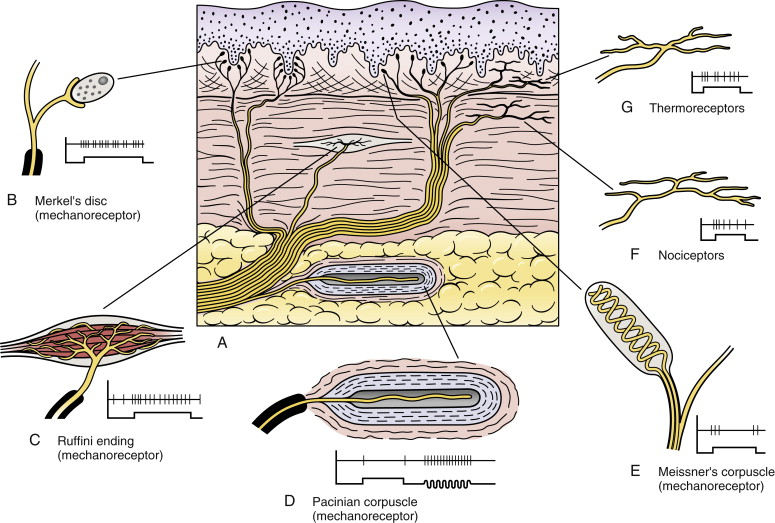
\includegraphics[width=0.45\textwidth]{img/skin.jpg}
\caption{Structure of a~skin. \cite{SkinStructure}\label{fig:skin}}
\end{center}    
\end{figure}

Some animals even use sensing the heat as~a~primary way how to~survive. Several groups of~snakes
(pythons, rattlesnakes, boas and others) use it when hunting warm-blooded animals (mouses, rats, rabbits etc.).
Blood-eating organisms (vampire bats, south-american heteroptera {\it Triatoma infestans})
have IR receptors to~look for a~vein under the skin.\cite{SnakeInfrared}


\paragraph{Discovery}
For the~first time, the~infrared electromagnetic waves were observed and named in 1800 by German-English
astronome sir Frederick Harschel. He dispersed light by a~prism and found out that the~temperature
of~the~light is growing with wavelength, the~red light had the~highest one.

When he measured the~temperature behind the red light, there was no~visible light on~the~table but
the~thermometer was showing even higher temperature moving beyond~the~red spectrum. Harshel
pronounced hypothesis that except the~visible light there must be also invisible one which we can~not
see. \cite{HerschelLife}

%\begin{figure}[h!]
%\begin{center}
%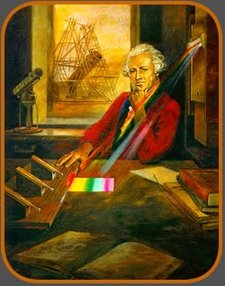
\includegraphics[width=0.4\textwidth]{img/herschel.jpg}
%\caption{Sir William Herschel discovering the~infrared radiation.\cite{HerschelLife}\label{fig:herschel}}
%\end{center}    
%\end{figure}

A~great coincidence is that he was an~astronome, he even discovered the~planet Uran, and it is his discovery,
the~IR waves, which now enables us to~explore and understand the~universe. \cite{NasaIrVideo}



\subsection*{Infrared radiation processed by machines}
\label{IRsensing}
PIR ({\it passive infrared}) sensor is an electronic device that scans electromagnetic
radiation at~wavelength $\lambda\in \langle 700~nm;2.5~mm \rangle$ aka frequency $f\in \langle 120~MHz;430~THz \rangle$. \cite{an2105}

\paragraph{Principles of PIR sensor}
There is a~number of approaches how to~construct such a~sensor. The~point is to~convert the electromagnetic
energy in~electric voltage and send it away via wire to~be processed by~hardware or~software.

First way how to do it is {\it a~bolometer}. It uses the fact that resistance of a~resistor is different
when changing a~temperature, as shown in the equation \ref{eq:bolo} for temperature difference $\Delta T$
and resistor with original resistance $R_0$ and new resistance $R_t$ and with temperature coefficient $\alpha$.
So with using the~same voltage it measures the~electric current and with the~Ohm law $R = \frac{U}{I}$
the~sensor computes instantaneus resistance.

\begin{equation}
\label{eq:bolo}
R_t = R_0 (1 + \alpha\Delta T)
\end{equation}

Another type is {\it a thermoelectric sensor} reacting to the different thermoelectric resistance of
exposed wire and comparative wire.

The~last is {\it a~pyroelectric detector}. The~principle is based on~electrostatic polarization,
changing during the~temperature change. \cite{DetectorsBook}

\begin{figure}[h!]
\begin{center}
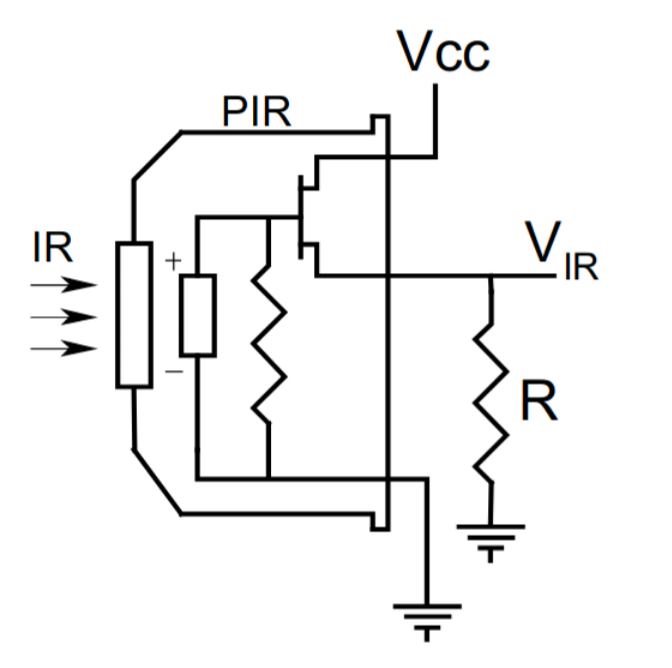
\includegraphics[width=0.25\textwidth]{img/pirscheme.png}
\caption{Single element pyroelectric detector.\cite{an2105}\label{fig:pir}}
\end{center}    
\end{figure}


\paragraph{Sensing of the infrared radiation}
The~structure of~PIR sensor is inspirated by structure of an~eye described in~subsection \ref{subsection:eye}.
An infrared ray incoming to the~sensor first goes through~{\it Fresnel lens} aiming it onto~a~pyroelectric sensor
as you can see in the~figure \ref{fig:fresnellens}. Then the~ray is transformed in an~electric voltage.

\begin{figure}[h!]
\begin{center}
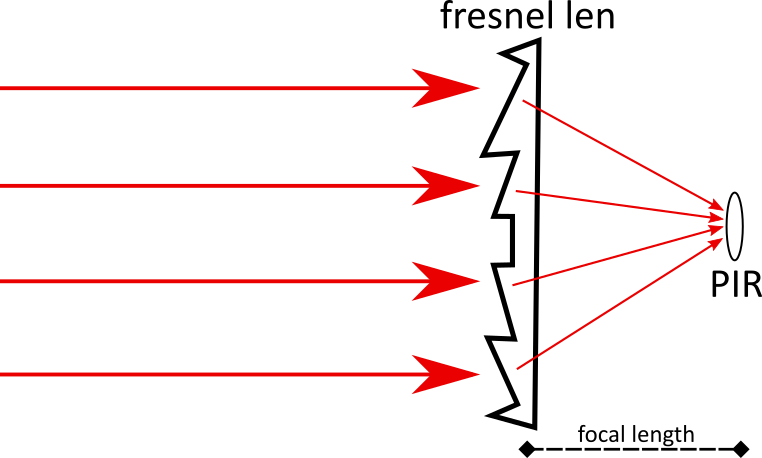
\includegraphics[width=0.3\textwidth]{img/fresnellens.png}
\caption{Fresnel lens.\label{fig:fresnellens}}
\end{center}
\end{figure}

Before the output the signal is being processed. For vast majority of application we are interested in
people sensing emitting radiation characterized in the figure \ref{fig:bodywavelength}.
Therefore the signal is amplified and filtered to well discriminate their presence and absence.
An example is a scheme \ref{fig:pirstd} of product {\it PIR STD} made by {\it B+B Sensors}.

\begin{figure}[h!]
\begin{center}
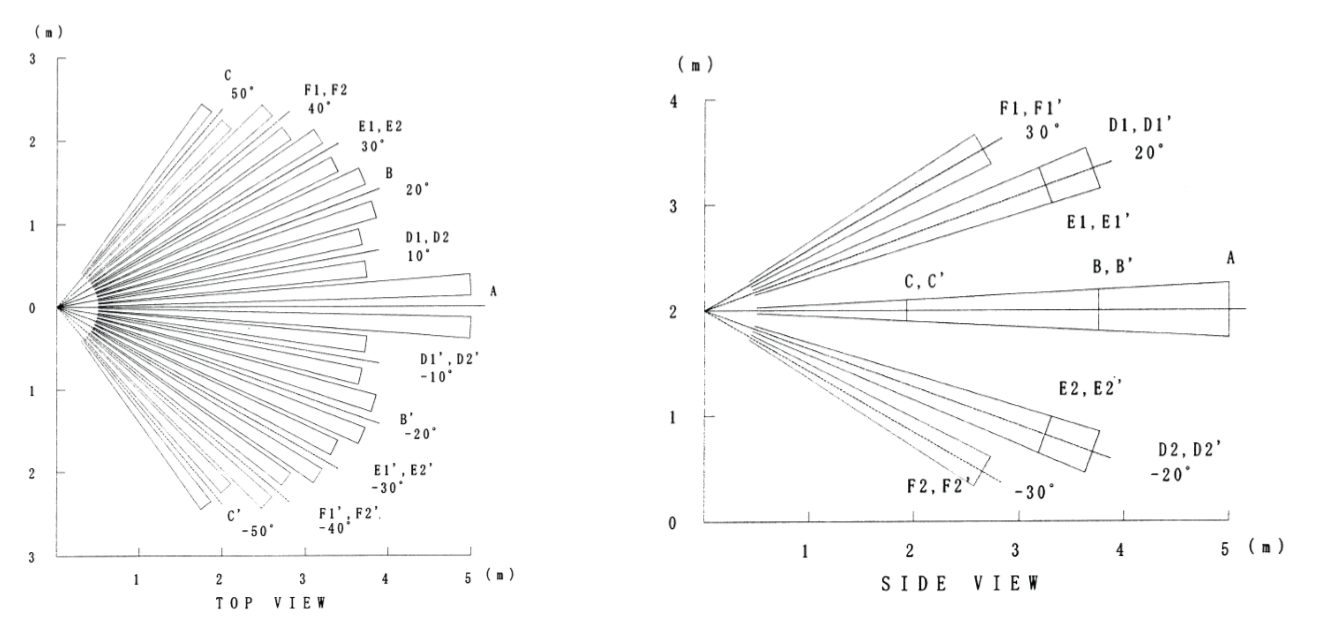
\includegraphics[width=0.7\textwidth]{img/roomsegments.png}
\caption{Sensing of PIR STD. \cite{PIROperationalManual}\label{fig:roomsegments}}
\end{center}    
\end{figure}



\newpage
\section{Pattern recognition}
The pattern recognition means processing of a signal and localizing of predefined objects.
The form is dependent on the type of signal and the objects that we search. Generally we can say
there are five parts of recognition pipeline.

\subsection*{Sensing}
In the world of digital computers sensing means {\it sampling}, converting a continuous signal
into discrete samples. It is present if the signal is being processed online.

Through different signal types various technologies for sensing are used -- image, sound, temperature,
pressure, weight, smell etc. The sensing procedure in the case of heat signal is described in the section
\ref{IRsensing}.

There is a few things that we need to deal during sensing: noise, linearity, callibration, ageing.

\subsection*{Segmentation}
The signal is splitted into segments by the time axis that are being processed separately. They can even overlap.
Segmentation ensures fast processing saving memory and other resources.

\subsection*{Features extraction}
Features are quantitive expression of the input signal, they replace the signal in the following phases.
Its purpose is to reduce memory and computational complexity of the processing. Each segment of $N$ samples
is transformed to vector of $K$ features, the point is to reduce dimensions, $K << N$, but preserve
relevant characteristics. Choosing the right features is therefore key for the following classifier.

To have good results the~features should be discriminative (distinguish between classes), invariant to
the transformations (translation, rotation, scale, deformation etc.) and decorrelated - mutually independent.

Vast number of described ways how to create features exists -- {\it Principal Component Analysis} (PCA),
{\it Linear Discriminant Analysis} (LDA). They can be used generally, but there is also many special
application-dependent features. 

\begin{figure}[h!]
\begin{center}
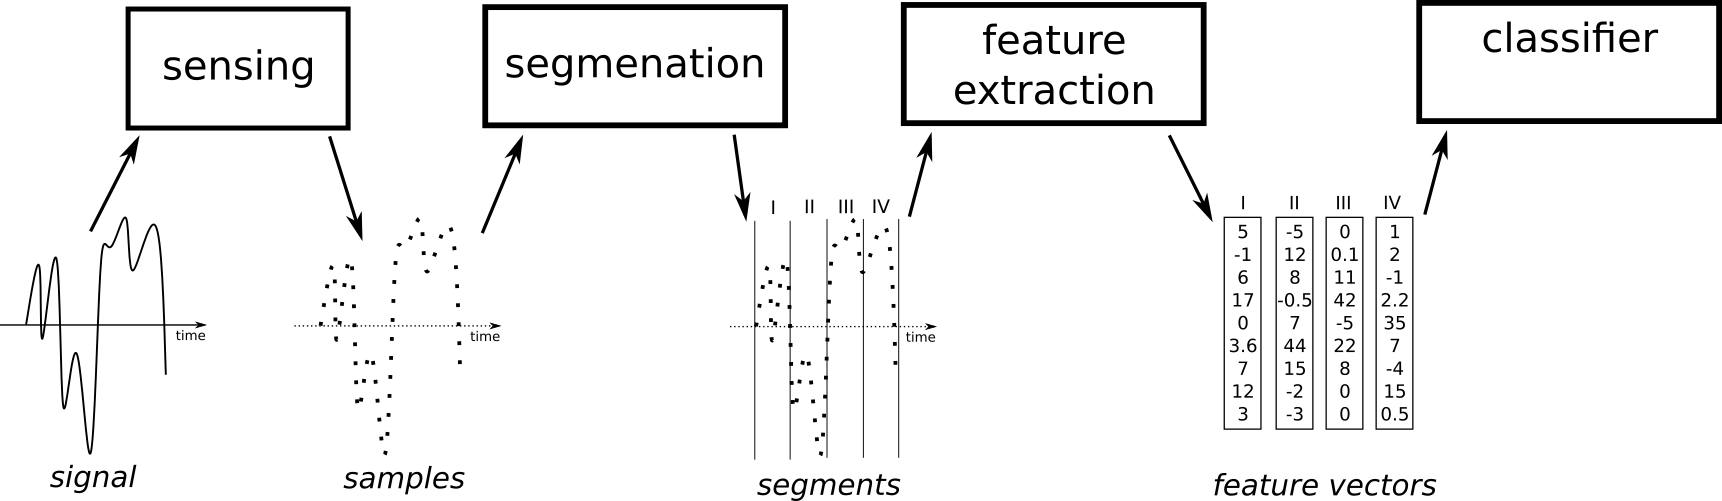
\includegraphics[width=0.7\textwidth]{img/featureextraction.png}
\caption{Preprocessing pipeline.\label{fig:featureextraction}}
\end{center}
\end{figure}

Multiple thesis and articles were written on the topic of heat signal processing. For the feature extraction,
\cite{SinglePIR} suggests {\it Wavelet Transformation}, \cite{ChirpletSVM} uses {\it chirplet}-based features,
but also tests other feature-extraction methods: PCA, Expanded-Class LDA or fusion of PCA and LDA feature vectors,
\cite{BayesanClassifier} calculates with the signal itself.

\subsection*{Classification}
Before we will describe the classification phase, several terms must be defined: 
\begin{itemize}
\item {\it Detection} is a~classifying of presence of observed object or~characteristic.
\item {\it Identification} is an~assigning the~observed object to~one of~$N$ classes.
\item {\it Detection Error Tradeoff} is a~relation of~miss to~false alarm probability of~a~classifier.
The~goal is minimizing both with finding the~best settings of~classifier parameters.
\end{itemize}
This thesis performs a detection of~a~presence of~a~person. In~the~case of~positive detection identification
of~the~situation is made -- what was actually detected and whether it is a~person or more people etc.

Finding the~most suitable classifier for~the~task is fundamental, but consequent to the~feature extraction
method we use. At~the~end of~the~day, inputs of~all the~methods is a~vector of~features for~each segment.
There are linear and non-linear classifiers, separating the~hyperdimentional space into~segments. Then
the~segment is detected or identified if features vector geometrically lies in~the right segment. 

It is also possible to~perform some kind of transformation before classification if the~space is not separable
linearly. But other attitudes are also possible like algorithm {\it K-nearest neighbors}.

An~output of a~classifier can be either a~hard decision or some~kind of soft score, which can be later processed
by a~postprocessor -- used to merge data from~more classifiers or something else. A~classical linear classifier
is used in {\it Linear Regression} or {\it Support Vector Machine} (SVM). Each neuron of recently very popular
{\it Neural Networks} (NN) can also be represented with linear classifier.

\begin{figure}[h!]
\begin{center}
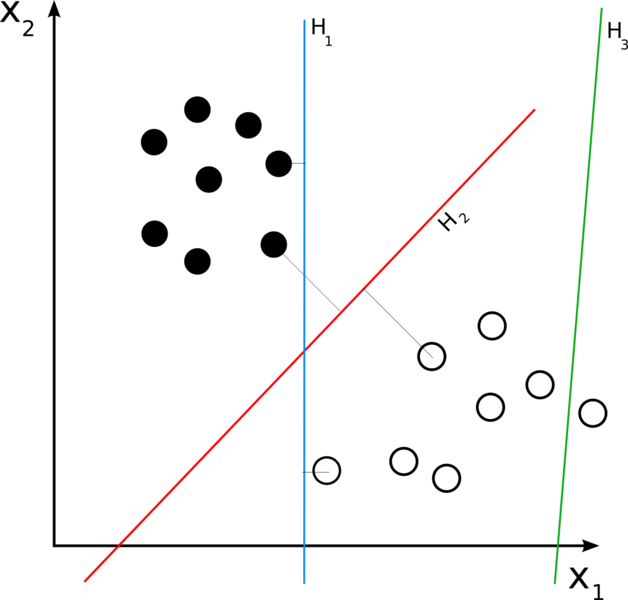
\includegraphics[width=0.3\textwidth]{img/linear.png}
\caption{Linear classifier.\cite{LinearClassifier}\label{fig:linearclassifier}}
\end{center}
\end{figure}

\subsection*{Postprocessing}
During postprocessing different information than pattern are used, procedure is
connected to the concrete task. This parts often includes hard decision, if the
classifier's output is a soft score -- prices are taken into consideration,
the simpliest way is using treshold.




\chapter{Design Description}

The design of the whole project is split in two products - sensing device
and the processing and visualising program - a server. Sensor measures signal
sensing the observed space with connected PIR sensor and sends the data. The server
collects the data from the sensor/sensors and performs the recognition of 
people and fusion algorithms over the results, if multiple sensors are connected.

Results might be displayed in the visualization program. The data are being sent
over network. In the implementation, LAN is used, but it could be possible to
use the Internet and send the data to the remote visualizer.


\section{Sensor device}

Heart of the sensing device is a preprogrammed MCU with PIR connected. Such device
uses AD convertor to read the signal value from the sensor. The device may also
perform fixed-sized segmentation in order to increase the effective data speed with
sending more samples within one chunk, but with regard to preserving {\it real-time}
nature.

One of the great issues, that needs to be solved is determining the position of the sensor,
or even worse -- mutual position of multiple sensors when used. Unless it is
known, no fusion can be done. If the intention is to sense the door area and count
number of incoming/outgoing people, then a position of the door needs to be known
in advance.

Very elegant solution is suggested in \cite{GestureControl}. Three PIR sensors are
places in fixed mutual position on a board, as shown in the figure \ref{fig:3pir_geometry}.
This brings several advantages, not only it increases the sensing angle,
but also solves problems with position of sensors, which is given by the board construction.
Such a construction is unsuitable to use in rooms though.

\begin{figure}[h!]
\begin{center}
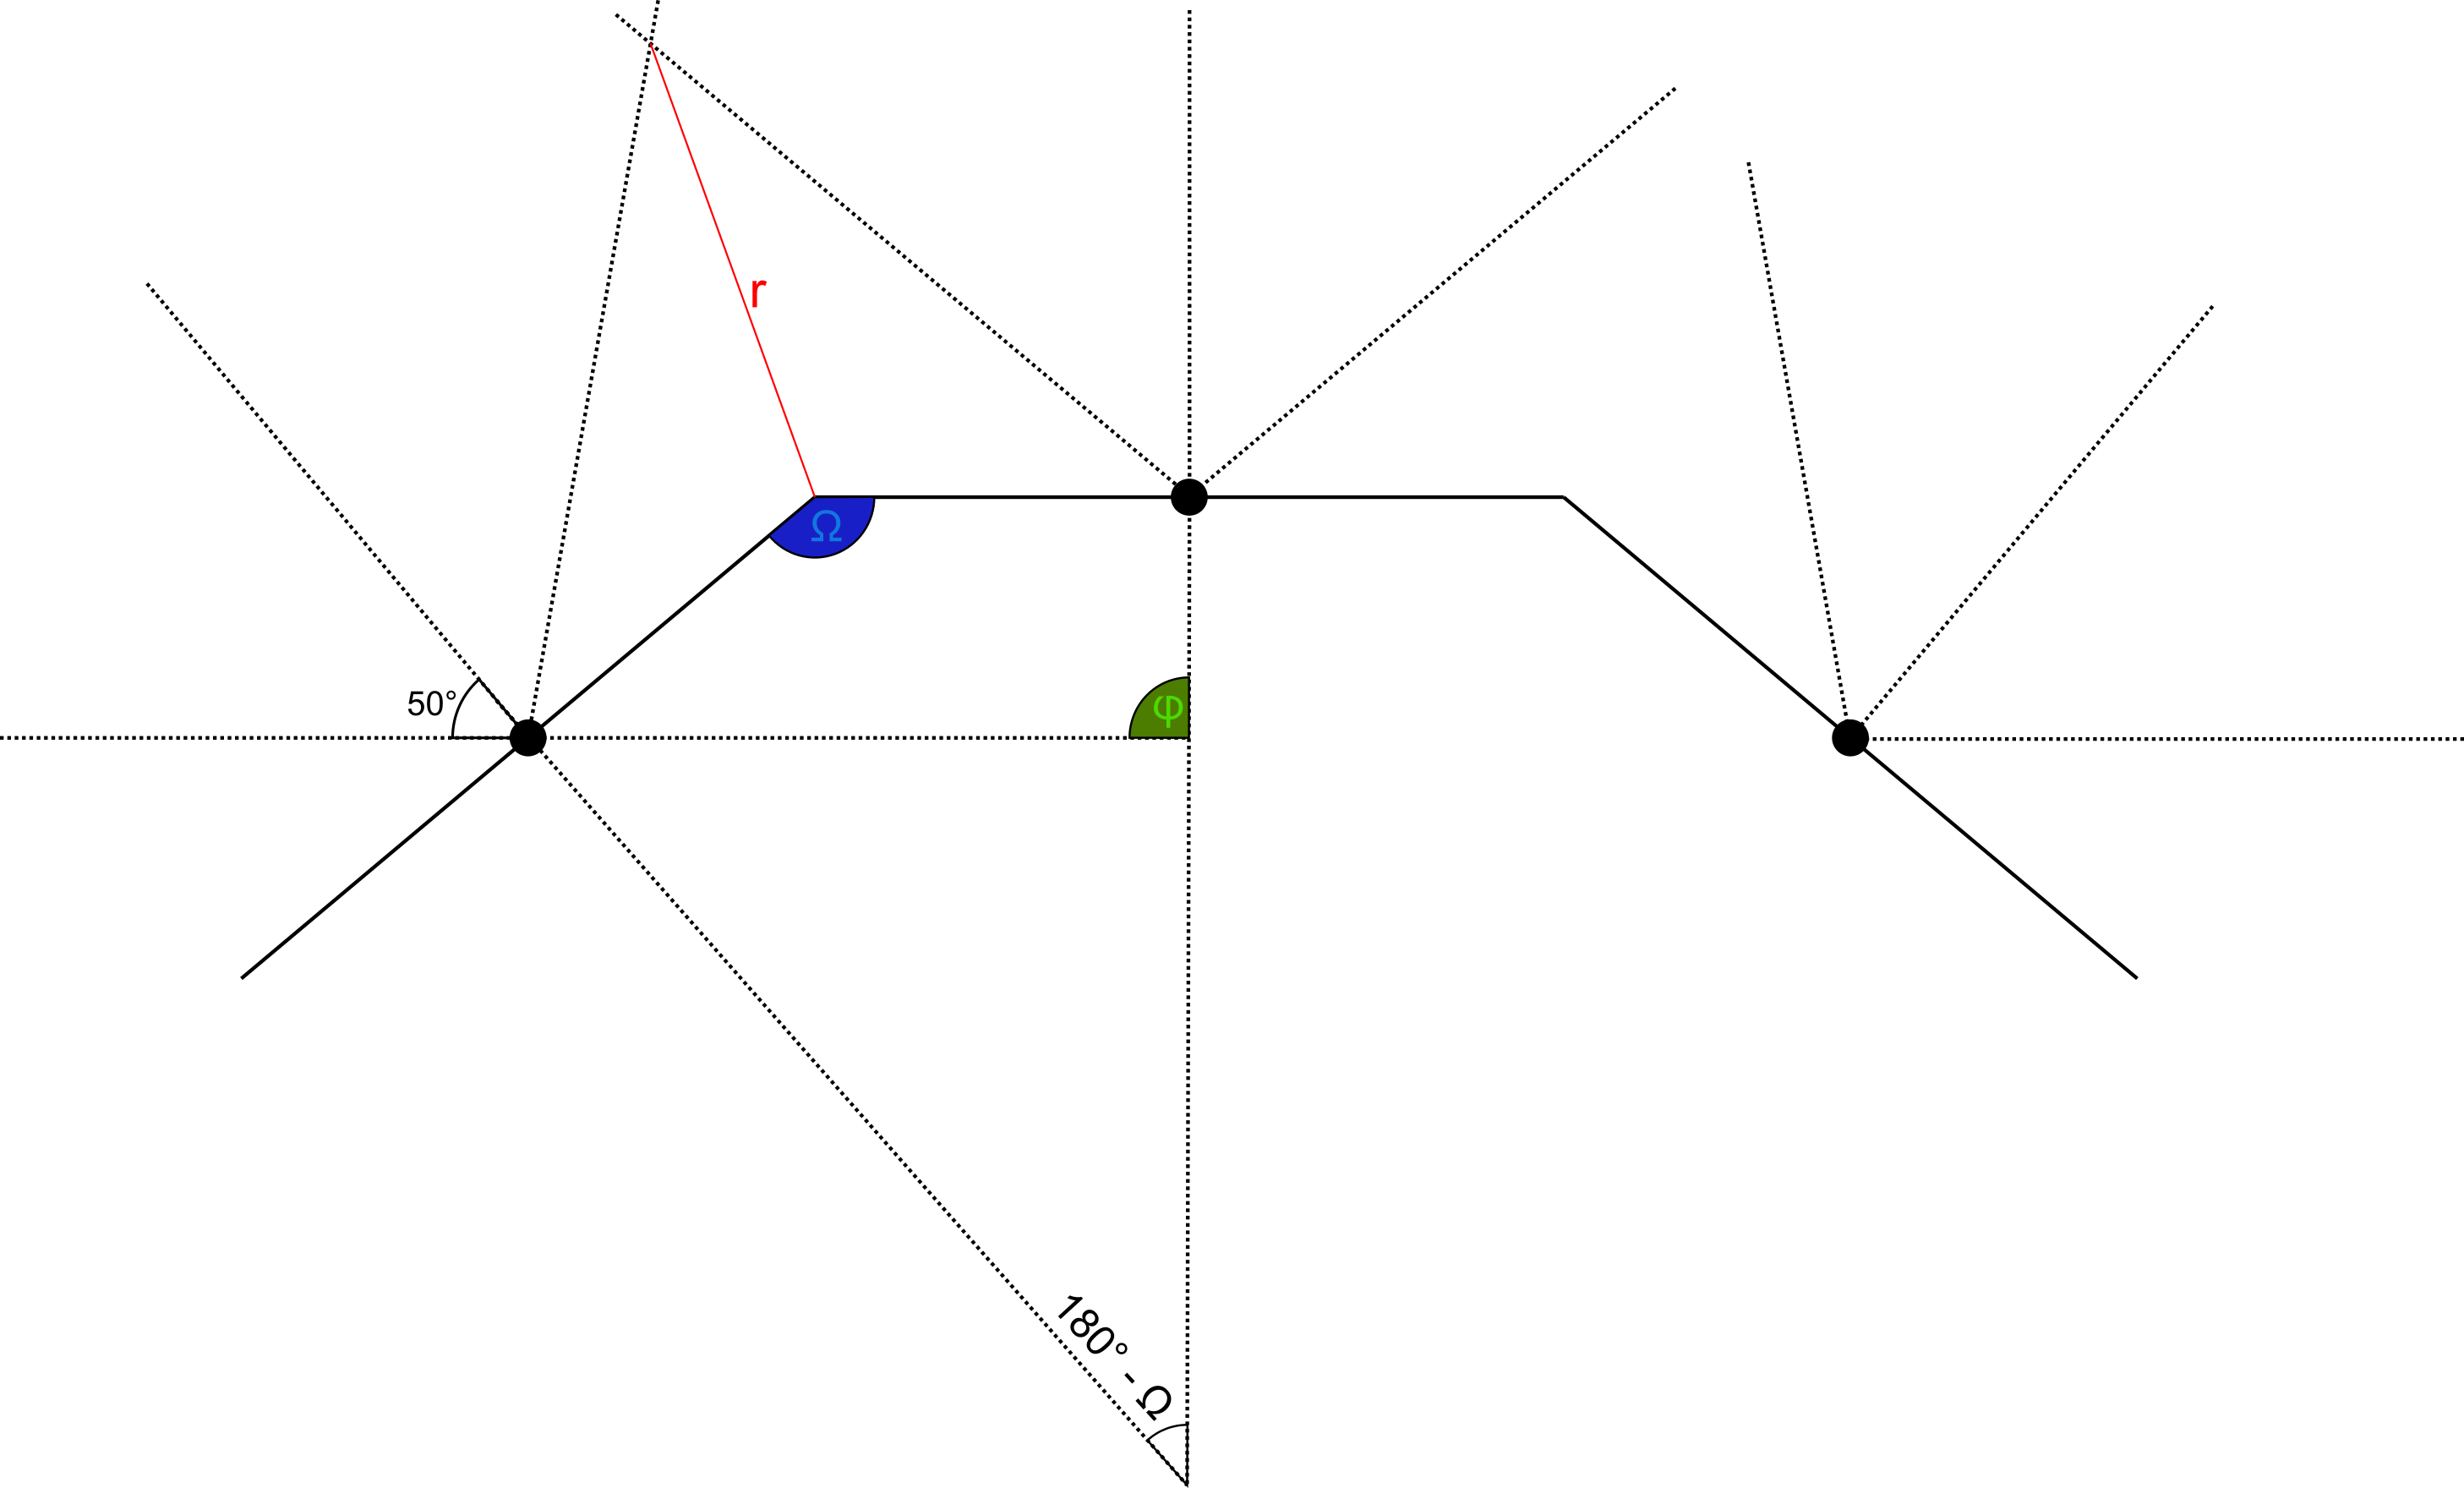
\includegraphics[width=0.4\textwidth]{img/3pir_geometry.png}
\caption{Geometry for three PIR sensors.\label{fig:3pir_geometry}}
\end{center}
\end{figure}

More flexible solution is probably inserting the dimension of space measured by the sensors
and their position directly to the fusion app as parameters. Issue of this is the positioning
itself. On the other hand, this solution can be easily extended with more parameters:
position of doors that can persons come or leave, windows and heaters that can have
unwanted influence and many others.

The device uses a serial communication channel, that can be read by the server. To
increase effectivity of the communication, the MCU sends the data in fixed period
as the chunk of fixed number of samples. The right size of the chunk must be chosen
with regard to the effectivity, but keeping the reaction fast enough. Sampling period and
sending period could be changed in the MCU configuration using REST API if the MCU
is reachable in a network and keeps a running web server.



%classification process described in subsection \ref{label:dataprocessing}.

%The sensors signal is at the end fused together and the results are classified objects
%with coordinates in polar coordinate system relative to the module position. These
%coordinates are sent to the client.

%The interior angle of module $\Omega$ is a parameter of the module construction. Using this parameter
%orientation $\lambda$ and position $p_X = (d_X,\varphi _X)$\footnote{Position uses polar coordinates
%with the origin in the central sensor.} of sensors can be expressed. Parameter $r$ is length
%of module edges with sensor in the center. Sensor PIR-STD by B+B Sensors has $250\times 250\times 200~\text{mm}$;
%therefore $r > 250~\text{mm}$.

%\begin{subequations}
%\begin{equation}
%\lambda_C = 0
%\end{equation}
%\begin{equation}
%\lambda_L = -\lambda_R = 180 - \Omega
%\end{equation}
%\end{subequations}

%\begin{subequations}
%\begin{equation}
%\varphi_C = 0
%\end{equation}
%\begin{equation}
%\varphi_L = -\varphi_R = 90 + \frac{180 - \Omega}{2}
%\end{equation}
%\end{subequations}

%\begin{subequations}
%\begin{equation}
%d_C = 0
%\end{equation}
%\begin{equation}
%d_L = d_R = \frac{r}{2} (r - 4cos(\Omega))
%\end{equation}
%\end{subequations}


\section{Classification server}
\label{section:classification}
On the used communication medium is running application listening to the channel.
This server parses the segments sent by the devices and performs the classification.


\subsection*{Artefact extraction and fuzzification}
The signal produced by the PIR has a specific nature, as it is shown in the appendix \label{appendix:PIRSignal}.
There are parts, that are constant, divided by abruptly changing edges, when there is a moving body. The
characteristics of the movement change character of the signal.

The signal first is segmented using {\it continuous wavelet transformation}
\footnote{
Continuous wavelet transformation is a signal processing technique transforming a signal to frequency domain.
The process is quite similar to fourier tranformation, instead of sinusoid it uses wavelet, a finite signal with
energy $E=0$, and therefore reacts better to abrupt changes.\cite{WaveletTour}}
with Morlet wavelet (\ref{eq:morlet})
and scale $s_{cwt} = 1.33846$, and the extrems are detected comparing to the $N_{n} = 8$ neighbors on both sides.
Detected extrems are used as the borders of the segments, that lies in between them. These numbers were
discovered experimentally minimizing the sum of the within-segment variances of the recorded data using formula \ref{eq:cwtparamssearch}



% Morlet "mexican hat" wavelet.
\begin{equation}
\Psi(x) = e^{-\frac{x^2}{2}} cos(5x)
\label{eq:morlet}
\end{equation}

% Experimental optimalization of parameters.
\begin{equation}
s_{cwt}, N_{n} = \text{argmin} ( \sum_{\sigma_i \in \sigma_{s,N}} \sigma_i )
\label{eq:cwtparamssearch}
\end{equation}

In the next step segment distances are evaluated. Distance of two adjoining segments aka {\it edge} is computed as numerical
difference of their within-segment mean values.

% Distance of segments or edge height.
\begin{equation}
||\textbf{AB}|| = \mu_\textbf{B} - \mu_\textbf{A}
\end{equation}

Here comes to the game fuzzification. A designed set of fuzzy membership functions $\xi_F$, $\xi_S$ and $\xi_R$
corresponds with artefacts falling edge (\textbf{F}), stagnating signal (\textbf{S}) and rising edge (\textbf{R}).
The E and R are related, they use the same wave form based on transformed $arctan()$ function, parametrizable with
tolerance $t$ and center/shift $x_0$. S is based on gaussian function. The fuzzy set arrange is visualized
in the figure \ref{fig:fuzzysets} with $t=10$.

% Fuzzy membership functions.
\begin{subequations}
\begin{equation}
\xi_R(x) = \frac{ arctan( 4\cdot (\frac{x - x_0}{t} + 1) )}{\pi} + 0.5
\end{equation}
\begin{equation}
\xi_F(x) = \xi_R(-x)
\end{equation}
\begin{equation}
\xi_R(x) = \sqrt{ exp( -\frac{(x_0 - x)^2}{2\cdot (0.6t)^2} ) }
\end{equation}
\end{subequations}


\begin{figure}[h!]
\begin{center}
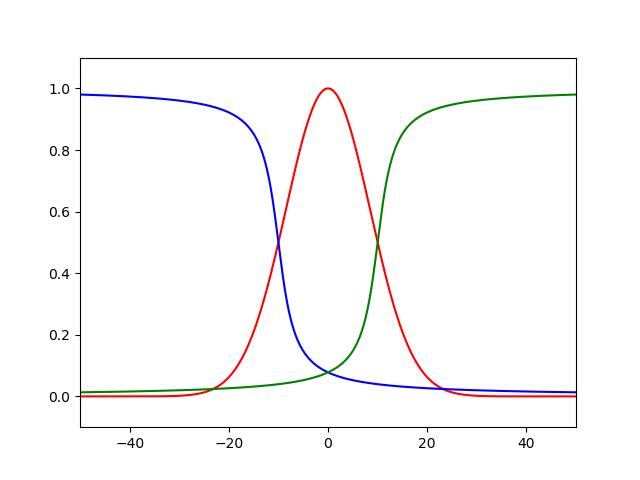
\includegraphics[width=0.6\textwidth]{render/fuzzysets.png}
\caption{Fuzzy sets used for fuzzification.\label{fig:fuzzysets}}
\end{center}
\end{figure}

Every edge gets assigned its fuzzy values for each of the classes. Now borders of artefacts need to be found.
Score of border $\xi[i]$ for the edge $x_i$ is evaluated using formula \ref{fig:artefactborder}.
\footnote{Operator $\land_P$ here means {\it product fuzzy T-norm}: $A \land_P B = f_A(x)\cdot f_B(x)$.}
The calculation is done for all the artefact combinations $ABC$ here, where $A$ is artefact of precedent $x_{i-1}$, $B$ for the
$x_i$ itself and $C$ for the follower $x_{i+1}$. $A,B,C \in \{F,S,B\}$.

% Artefact combination fuzzy formula.
\begin{equation}
\xi_{ABC}[i] = (\xi_{A}[i-1]) \land_P (\xi_{B}[i]) \land_P (\xi_{C}[i+1])
\label{fig:artefactborder}
\end{equation}

The combination indicating artefact border are put together as same as the rest. That is reached
using formula \ref{eq:edgemerger}.\footnote{Operator $\lor_{p\Sigma}$ here means
{\it probability sum fuzzy S-norm/T-conorm}: $A \lor_{p\Sigma} B = f_A(x) + f_B(x) - f_A(x)f_B(x)$.
Other variants could be considered too - maximum, Lukasiewicz, etc. } Border indicating
combinations are those, whose precedent and own combination differ, aka. {\it \{SF*, FS*, RF*, FR*, RS*, SR*\} }.
The rest, {\it \{FF*, SS*, RR*\}}, means no edge. The results are tresholded for $T = 0.5$.

% Artefact border fuzzy formula.
\begin{subequations}
\begin{equation}
f_{1}[i] = \bigvee\limits_{\xi \in \xi_1}{}_{p\Sigma} (\xi)
\end{equation}
\begin{equation}
f_{0}[i] = \bigvee\limits_{\xi \in \xi_0}{}_{p\Sigma} (\xi)
\end{equation}
\label{eq:edgemerger}
\end{subequations}


Newly created artefacts will be used to form feature vectors, filled with each one's characteristics.
Suggested metrics are variance and mean value of samples within artefact, scope of line, that 
can be counted using formula \ref{eq:artefactline}, etc.
$l_0$, $l_1$ are $y$ coordinates of first and last point of the line respectively,
\textbf{A} is a artefact samples vector. $k$ is the searched line scope,
$\Delta_{\textbf{A},k}$ is the difference score of artefact \textbf{A} and line with scope
$k$. It can also be used as a feature. This representation is to be seen in the figure \ref{fig:siglines}.

\begin{subequations}
\begin{equation}
l[i] = k\textbf{A}[i] + l_0
\end{equation}
\begin{equation}
k = \frac{l_1 - l_0}{|\textbf{A}|}
\end{equation}
\begin{equation}
\Delta _{\textbf{A},k} = \sum_{i \in \{1,...,|\textbf{A}|\}} (\textbf{A}[i]-l[i])^2
\end{equation}
\begin{equation}
l_0,l_1 = \text{argmin} ( \Delta_{\textbf{A},k} )
\end{equation}
\label{eq:artefactline}
\end{subequations}

\begin{figure}[h!]
\begin{center}
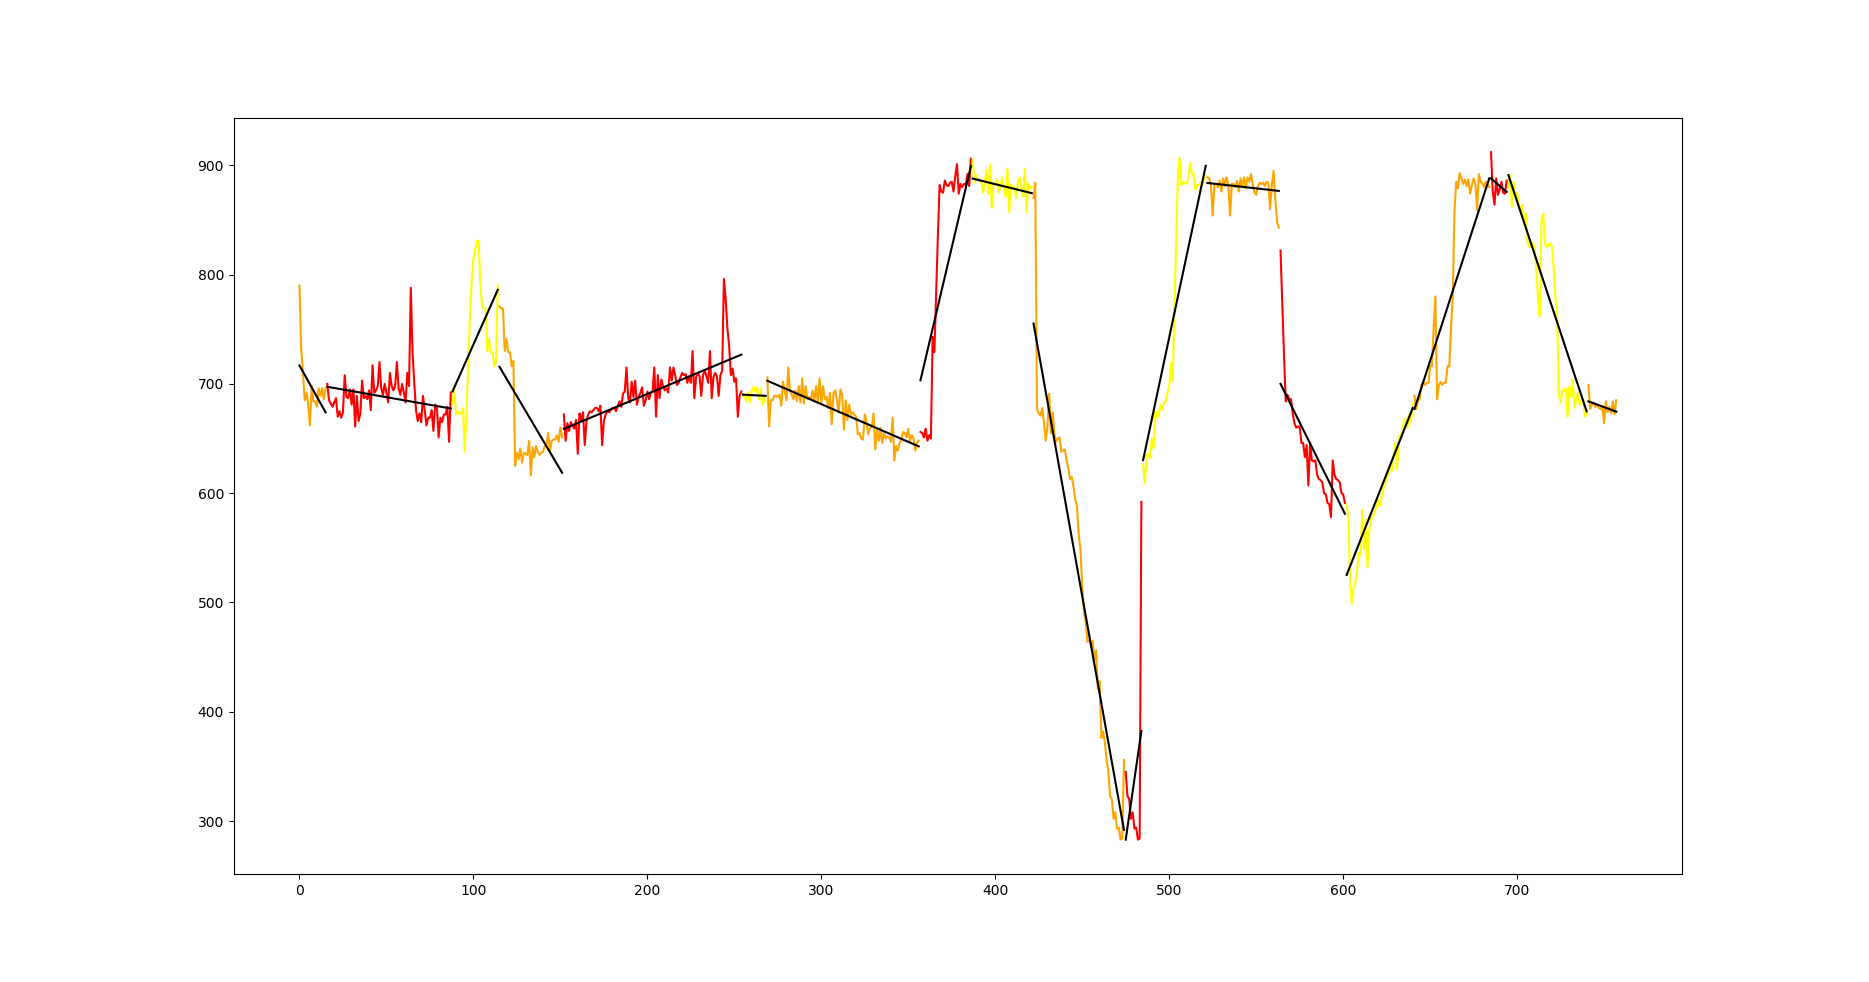
\includegraphics[width=0.85\textwidth]{render/signallines.png}
\caption{Representation of artefacts using line scope.\label{fig:siglines}}
\end{center}
\end{figure}

\subsection*{Classification}
Extracted feature vectors for every detected artefact will undergo classification procedure
consisting of multiple dichotomic classifiers, each evaluating single decision - whether
the movement is present or not, if the movement is towards center or aside, if the
movement is closer to sensor of far, and if possible, if the person is on the left side
or right.

The classification is process based on linear regression, searching for the best linear
separation of the training data using linear classifier \ref{eq:linearclassifier}, where 
$\overline{x}$ is an input, $\sigma(a)$ is activation function mapping
$\mathbb{R} \rightarrow \langle 0;1\rangle$ and $\overline{w}$,$w_0$ are searched parameters
of the classifier.


\begin{equation}
y(x) = \sigma (\overline{w}^T \overline{x} + w_0)
\label{eq:linearclassifier}
\end{equation}

The estimation of classifier's parameters $\overline{w}$,$w_0$ means maximizing the
posterior probabilities of each training data as same as solving the equation
\ref{eq:regressionEq}, in the logarithm domain \ref{eq:regressionLog}.

\begin{subequations}
\begin{equation}
p(t|\textbf{X}) = argmax \prod_{n \in C_1}y(\overline{x}_n) \prod_{n \in C_2} \{ 1 - y( \overline{x}_n ) \}
\label{eq:regressionEq}
\end{equation}
\begin{equation}
-\text{ln}( p(t|\textbf{X}) ) = - \sum_{n=1}^N \{ (t_n)\text{ln}(y_n) + (1-t_n)\text{ln}(1-y_n) \} = E(\overline{w})
\label{eq:regressionLog}
\end{equation}
\end{subequations}

The searched extrem of \ref{eq:regressionLog} means derivation \ref{eq:regressionGradient}
equal to $0$, solved numerically using \ref{eq:regressionGradientNumerical}.
$\eta \in (0;1\rangle$ is a converging parameter, the computation can be stopped either after
fixed step count or using minimal solution improvement $\varepsilon < | w^{(\tau + 1)} - w^{(\tau)} |$.

\begin{subequations}
\begin{equation}
\nabla E(\overline{w}) = \sum_{n=1}^N (y_n - t_n)x_n = 0
\label{eq:regressionGradient}
\end{equation}
\begin{equation}
w^{(\tau + 1)} = w^{(\tau)} - \eta \nabla E(\overline{w})
\label{eq:regressionGradientNumerical}
\end{equation}
\end{subequations}

The classifier's output is a 2D fuzzy value matrix, representing the space in from of the sensor.
It is inspired by the space representation by cellular automata, which carves it into small
homogenous segments. The fuzzy value at certain index expresses a presence of a person
at the position. Even though the space because of the construction of sensor has a shape of
circular sector, it can be easily represented by classical 2D matrix, as it is shown in the figure \ref{fig:circularsector}.

\begin{figure}[h!]
\begin{center}
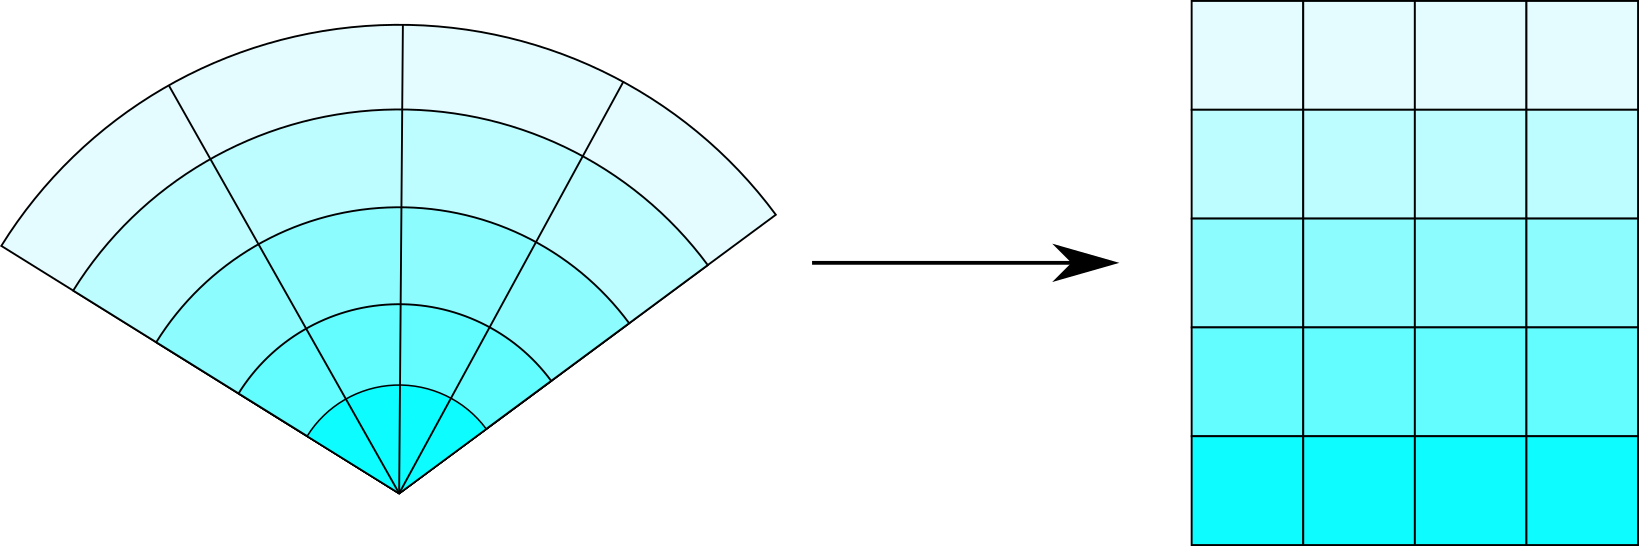
\includegraphics[width=0.5\textwidth]{img/circularsector_transformation.png}
\caption{Representation of circular sector.\label{fig:circularsector}}
\end{center}
\end{figure}

Each of the scores is fuzzified using sigmoid function and merged together using formula \ref{eq:regressionmerger},
creating the resulting matrix, as shown in the figure \ref{fig:areamatrixweighting}. {\it Consider action characteristics (speed, direction, multiple people) and state engine.}

\begin{equation}
TODO
\label{eq:regressionmerger}
\end{equation}



\begin{figure}[h!]
\begin{center}
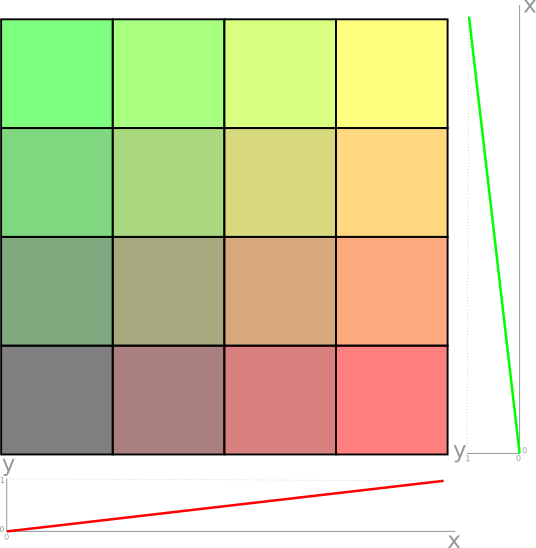
\includegraphics[width=0.3\textwidth]{img/pir_area.png}
\caption{Weighting of regression score to area matrix.\label{fig:areamatrixweighting}}
\end{center}
\end{figure}

\subsection*{Fusion}
Using more sensors brings advantages: the measuring might be more precise since the person presence
classified by two independent sensors is not only more probable but the computed position
can get more accurate than when using only one sensor. The disadvantage is higher price and need
to know the mutual orientation and position of the sensors. 

%If more sensors are used it is necessary to merge their space segments matrixes in one,
%as shown in the figure \ref{fig:3pir_area}. To do so, a fuzzy logic mechanism
%{\it Takagi-Sugeno rules} can be used as described in \cite{InsightIntoFuzzyModelling}.
%The form of rules is [IF {\it antecendent} THEN {\it succendent}] as shown in the table
%\ref{table:takagisugeno}. During the calculation all the antecendentes are evaluated
%and the most relevant leads to application of corresponding succendent to the output.

%\begin{figure}[h!]
%\begin{center}
%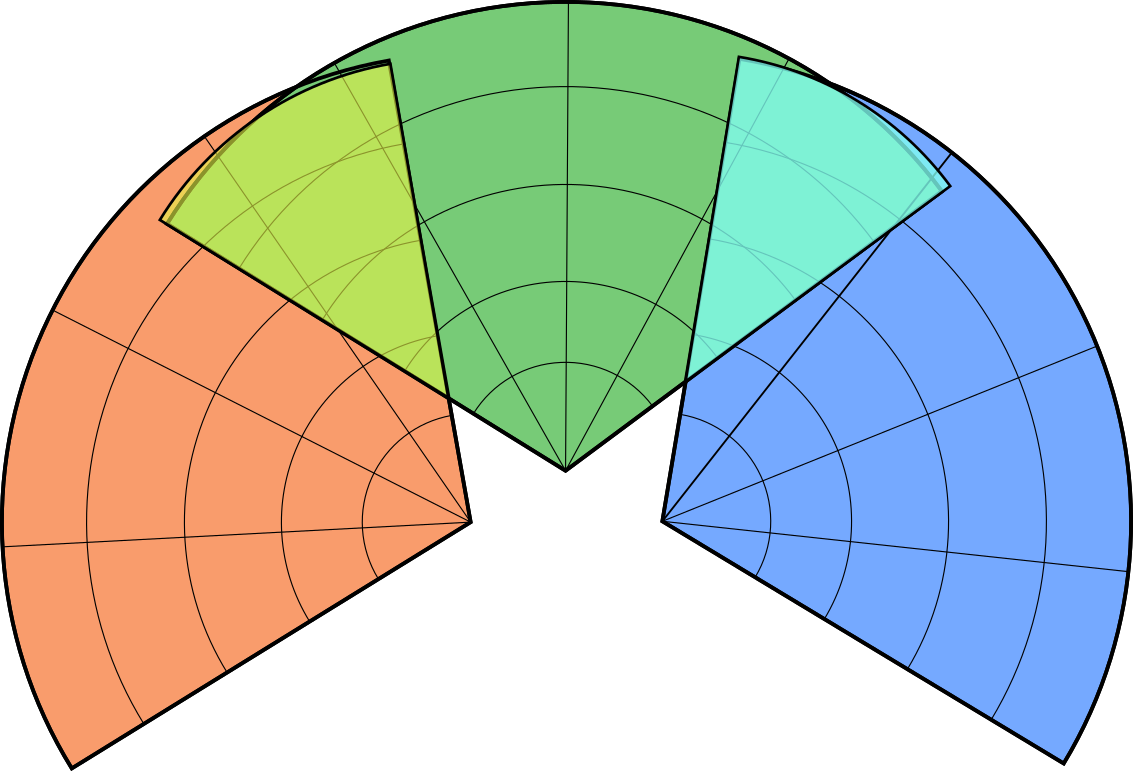
\includegraphics[width=0.5\textwidth]{img/3pir_area.png}
%\caption{Fusion of detection areas.\label{fig:3pir_area}}
%\end{center}
%\end{figure}

%\begin{table}[h!]
%\begin{center}
%\begin{tabular}{|c|c|c|} \hline
%\textbf{Rule}   & \textbf{Antecendent}                                & \textbf{Succendent}                             \\ \hline
%$R_1$           & $X_1$ is $A_{11}$ and \dots and $X_n$ is $A_{1n}$   & $Y = b_{10} + b_{11}X_1 + \dots + b_{1n}X_n$    \\ \hline
%$R_2$           & $X_1$ is $A_{21}$ and \dots and $X_n$ is $A_{2n}$   & $Y = b_{20} + b_{21}X_1 + \dots + b_{2n}X_n$    \\ \hline
%\multicolumn{3}{|c|}{\dots}                                                                                             \\ \hline
%$R_m$           & $X_1$ is $A_{m1}$ and \dots and $X_n$ is $A_{mn}$   & $Y = b_{m0} + b_{m1}X_1 + \dots + b_{mn}X_n$    \\ \hline
%\end{tabular}
%\caption{Takagi-Sugeno rules. $X$ is input, $A$ is a matrix of fuzzy numbers, $b$ is a matrix of fuzzy coefficients.\label{table:takagisugeno} \cite{InsightIntoFuzzyModelling}}
%\end{center}
%\end{table}

%The designed fusion fuzzy system is to be seen in the table \ref{table:fuzzyfusion}. To be able to merge
%the space segments, overlap must be known and then vector $X$ is created, containing pairs of values
%from each vector ($X[i]_L$ and $X[i]_R$). Each of these pairs is input to the fusion algorithm, which
%merges it to one fuzzy number result. 

%$C_{L}$ and $C_{R}$ are 2D matrixes of coefficients with indexing $[i,j]$, where $i,j \in \{0,L,M,H\}$.
%The fuzzy sets LOW, MEDIUM and HIGH of $X$ composes a basic evaluative trichotomy extended for unknown state OUT.
%The optimal values of coefficients and the fuzzy sets parameters have to be found experimentally. 

%\begin{table}[h!]
%\begin{center}
%\begin{tabular}{|c|c c|rcl|} \hline
%\textbf{Rule}   & \textbf{$X_L$}  & \textbf{$X_R$}  & \multicolumn{3}{|c|}{\textbf{Y}}  \\ \hline
%$R_1$           & OUT             & OUT             & $C_{L}[0,0]    $&+&$ C_{R}[0,0]   $   \\ \hline
%$R_2$           & OUT             & LOW             & $C_{L}[0,L]    $&+&$ C_{R}[L,0]X_R$   \\ \hline
%$R_3$           & OUT             & MEDIUM          & $C_{L}[0,M]    $&+&$ C_{R}[M,0]X_R$   \\ \hline
%$R_4$           & OUT             & HIGH            & $C_{L}[0,H]    $&+&$ C_{R}[H,0]X_R$   \\ \hline
%$R_5$           & LOW             & OUT             & $C_{L}[L,0]X_L $&+&$ C_{R}[0,L]   $   \\ \hline
%$R_6$           & LOW             & LOW             & $C_{L}[L,L]X_L $&+&$ C_{R}[L,L]X_R$   \\ \hline
%$R_7$           & LOW             & MEDIUM          & $C_{L}[L,M]X_L $&+&$ C_{R}[M,L]X_R$   \\ \hline
%$R_8$           & LOW             & HIGH            & $C_{L}[L,H]X_L $&+&$ C_{R}[H,L]X_R$   \\ \hline
%$R_9$           & MEDIUM          & OUT             & $C_{L}[M,0]X_L $&+&$ C_{R}[0,M]$      \\ \hline
%$R_{10}$        & MEDIUM          & LOW             & $C_{L}[M,L]X_L $&+&$ C_{R}[L,M]X_R$   \\ \hline
%$R_{11}$        & MEDIUM          & MEDIUM          & $C_{L}[M,M]X_L $&+&$ C_{R}[M,M]X_R$   \\ \hline
%$R_{12}$        & MEDIUM          & HIGH            & $C_{L}[M,H]X_L $&+&$ C_{R}[H,M]X_R$   \\ \hline
%$R_{13}$        & HIGH            & OUT             & $C_{L}[H,0]X_L $&+&$ C_{R}[0,H]   $   \\ \hline
%$R_{14}$        & HIGH            & LOW             & $C_{L}[H,L]X_L $&+&$ C_{R}[L,H]X_R$   \\ \hline
%$R_{15}$        & HIGH            & MEDIUM          & $C_{L}[H,M]X_L $&+&$ C_{R}[M,H]X_R$   \\ \hline
%$R_{16}$        & HIGH            & HIGH            & $C_{L}[H,H]X_L $&+&$ C_{R}[H,H]X_R$   \\ \hline
%\end{tabular}
%\caption{Design fuzzy system to fuseTakagi-Sugeno rules. $X$ is input, $A$ is a matrix of fuzzy numbers, $b$ is a matrix of fuzzy coefficients.\label{table:fuzzyfusion} \cite{InsightIntoFuzzyModelling}}
%\end{center}
%\end{table}

%For three sectors as in the figure \ref{fig:3pir_area} the situation is analogous. The table also depends
%on whether the areas of the side sensors overlap or not. Or they can be merged successively.

\subsection*{Defuzzification}

To get the results in a form of coordinate(s) of classified objects a cluster analysis is done. It calculates
a clusters of high membership values, for optimalization $\alpha$-cut on a certain level or tresholded
matrix can be used. Algorithm PAM (Partitioning Around Medoids is used), similar to k-means, where item called
medoid is used to represent the cluster instead of mean.

\begin{equation}
\mathit{PAM}(k, data) = argmin \left( \sum_{i=1}^{k} \sum_{j=1}^{k} ||data_{i} data_{j}||  \right)
\end{equation}

\begin{lstlisting}[style=python]
def PAM(k,data):
  # pick medoids
  medoids = [].generate(k,data.random())
  # compute dissimilarity matrix
  dm = DissimilarityMatrix(data,calculateDistance)
  # create clusters
  changed = True
  while changed:
    changed = False
    clusters = []
    for medoid_idx,medoid in medoids.enum():
      cluster = []
      for d in data:
        # add to cluster with closest distance to its medoid
        if dm[d,medoid] == dm[d,medoids].min():
          cluster.append(d)
      # set new center (SWAP phase)
      cluster.append(medoid)
      if medoid is not cluster.center():
        medoids[medoid_idx] = cluster.center()
        changed = True
      clusters.append(cluster)
  return clusters
\end{lstlisting}

\begin{lstlisting}[style=python]
function elbow(data):
  # try all k
  best = inf
  for k in <1,K_MAX>:
    clusters = PAM(data, k)
    # take minimal
    if WCSS(clusters) < best:
      best = clusters
  return best
\end{lstlisting}

To estimate the $k$, elbow method can be used: calculating k-means for different k values and taking the one with
minimal within-cluster sum of square (WCSS).\cite{ClusterAnalysis} \cite{VagueNatureInformation}

\begin{equation}
\mathit{WCSS} = \sum_{i=1}^{k} \sum_{x \in S_i} ||x - \mu_i||^2
\end{equation}

Very important is computing a distance of two segments. Since the original circular sector segmentation
is not homogenous, the distances varies with each distance. It can be calculated though using
cosine law. $P = (d, \alpha)$ is a segment given by polar coordinates, $d$ is distance and $\alpha$ is
azimuth.

\begin{equation}
|P_{1} P_{2}| = \sqrt{(d_{1})^{2} + (d_{2})^{2} - 2d_{1}d_{2}(\alpha_1 - \alpha_2)}
\end{equation}




\chapter{Data}

A output of a sensor as you can see in the figures \ref{fig:signalcalm} and \ref{fig:signalwalk}
is very discriminative -- with a bare eye a movement from no movement is distinguishable.
A detection of presence used in light sensors can be implemented with tresholding, this attitude is
not very suitable for classification of anything else except the presence itself.

In a calm state the sensor sends a constant signal\footnote{Constant signal in the terms
of electricity, slightly polluted with a background noise etc.}. Movement in the sensed area causes
abrupt changes of output. When the object either leaves the area, or stays completely calm, the signal
changes are getting slower and after a little while the output voltage gets in the calm state again.

\begin{figure}[h!]
\begin{center}
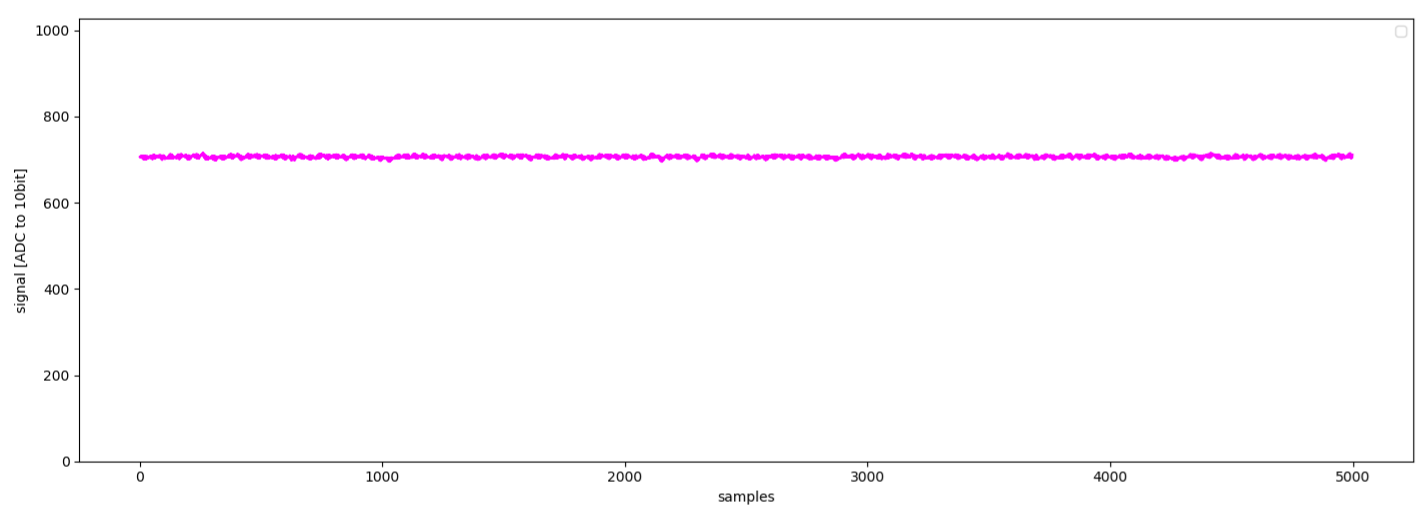
\includegraphics[width=0.65\textwidth]{render/signal_calm.png}
\caption{Signal of zero movement.\label{fig:signalcalm}}
\end{center}
\end{figure}

\begin{figure}[h!]
\begin{center}
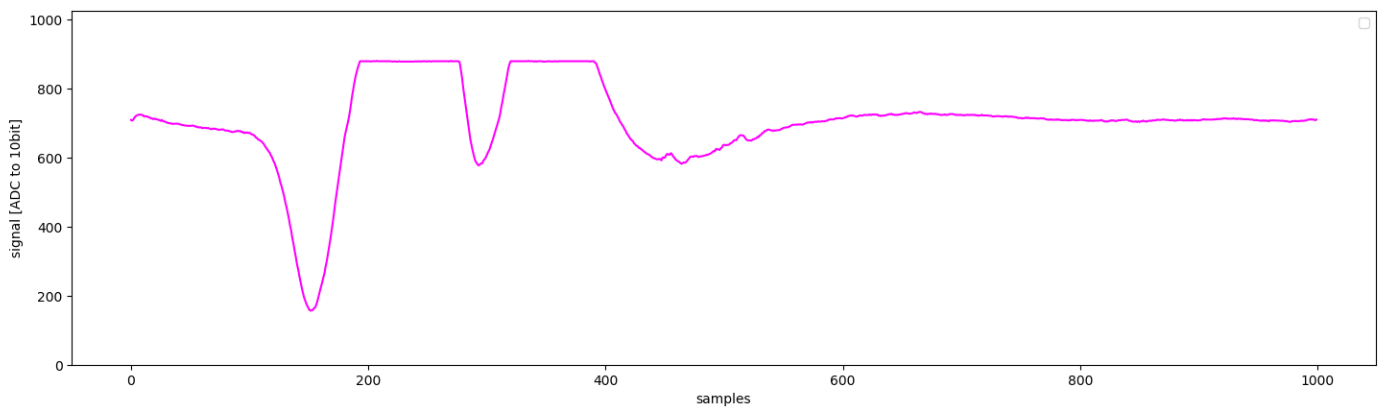
\includegraphics[width=0.65\textwidth]{render/signal_walk.png}
\caption{Signal of person walking around.\label{fig:signalwalk}}
\end{center}
\end{figure}

Therefore, the nature of the signal does not seem to need a complicated method to perform a classification on it.
{\it Fourier transformation} and {\it wavelet transformation} were considered for feature
extraction. The abrupt changes in the signal could be problem for FT, because it can not represent
it efficiently\cite{SinglePIR}, % youtube video
but unlike sinusoids, the wavelets exist for a finite duration and they are suitable for representing
abrupt changes.

The wavelet transformation is defined as a function $F_{(s,k)}(x)$. Parameters s,k are scale and shift, changing
them in predefined unit and interval creates a matrix, as you can see in the figure \ref{fig:walk03}.

\begin{equation}
F_{(s,k)}(x) = \sum_{n=1}^{N} x[n] \Psi_{(s,k)}^{*}[n]
\end{equation}

Firstly The data were offline analysed using {\it Matlab}, which has implemented wavelet transformation.
The Matlab is not used because it is proprietary software and the program would be dependent on it.
During the analysis it was found, that the data are very well separable using continuous wavelet tranformation.

\begin{figure}[h!]
\begin{lstlisting}[style=matlab]
data = csvread('walk02.csv');
wscalogram('image', cwt(data));
\end{lstlisting}
\caption{Matlab code performing cwt.\label{list:cwtmatlab}}
\end{figure}

\begin{figure}[h!]
\begin{center}
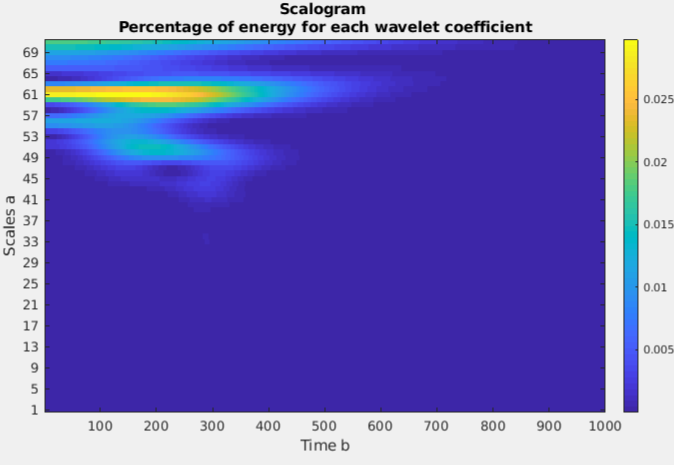
\includegraphics[width=0.5\textwidth]{img/walk03.png}
\caption{Matlab {\it cwt()} output of {\it walk03.csv}.\label{fig:walk03}}
\end{center}
\end{figure}


The training and testing data were recorded as a part of the work, results are
shown and described by the appendix \ref{appendix:PIRSignal}.




\chapter{Implementation}

\section{Sensor device}

The sensor device consists of PIR sensor and programmed MCU that samples analog signal from
sensor and writes in chunks called segments it via WiFi to local multicast group.

Nowadays most of the PIR sensors sold have only a binary {\it switching} output.
When signal reaches a set treshold output is set to logic "1" for a unit of time.
This mechanism is suitable for a light sensor or door sonsor, completely useless
for the needs of this project though.

The only found sensor that offers an analog output was {\it PIR STD} by
{\it B+B Sensors}.

\subsection*{PIR STD}
{\it PIR STD} is a product of {\it B+B Sensors}. It is the only found passive infrared
sensor, that has except of the switching binary ouput also analog output. Except of
operating voltage $V_{cc}$ and ground $GND$ pins, it also has reference voltage input,
which needs to be connected to $\frac{V_{cc}}{2} V$. The optical resistance pins can
be also used for additional classification, fusion with the infrared signal classification
results and making the final result more accurate.

Pin layout table from the sensor operational manual is shown in the table \ref{fig:pirstdpin}.

\begin{table}[h!]
\begin{center}
\begin{tabular}{|c c | c | c |} \hline
\textbf{Pin} & \textbf{Code} & \textbf{Type} & \textbf{Description} \\ \hline
1 & ANA & O & Analog output \\ \hline
2 & REF & I & Reference voltage \\ \hline
3 & GND & O & Ground \\ \hline
4 & OUT & O & Binary (switching) output \\ \hline
5 & GND & O & Ground \\ \hline
6 & VCC & I & Operating voltage \\ \hline
7 & LDR & O & Optical resistance \\ \hline
8 & LDR & I & Optical resistance \\ \hline
\end{tabular}
\end{center}
\caption{Pin layout of PIR STD.\cite{PIROperationalManual}\label{fig:pirstdpin}}
\end{table}

The {\it PIR STD} scheme shown in the figure \ref{fig:pirstdscheme} processes the signal
in three stages going from left to right. The first two filter and amplify the signal
resulting with analog output. The third generates binary output from analog.

\begin{figure}[h!]
\begin{center}
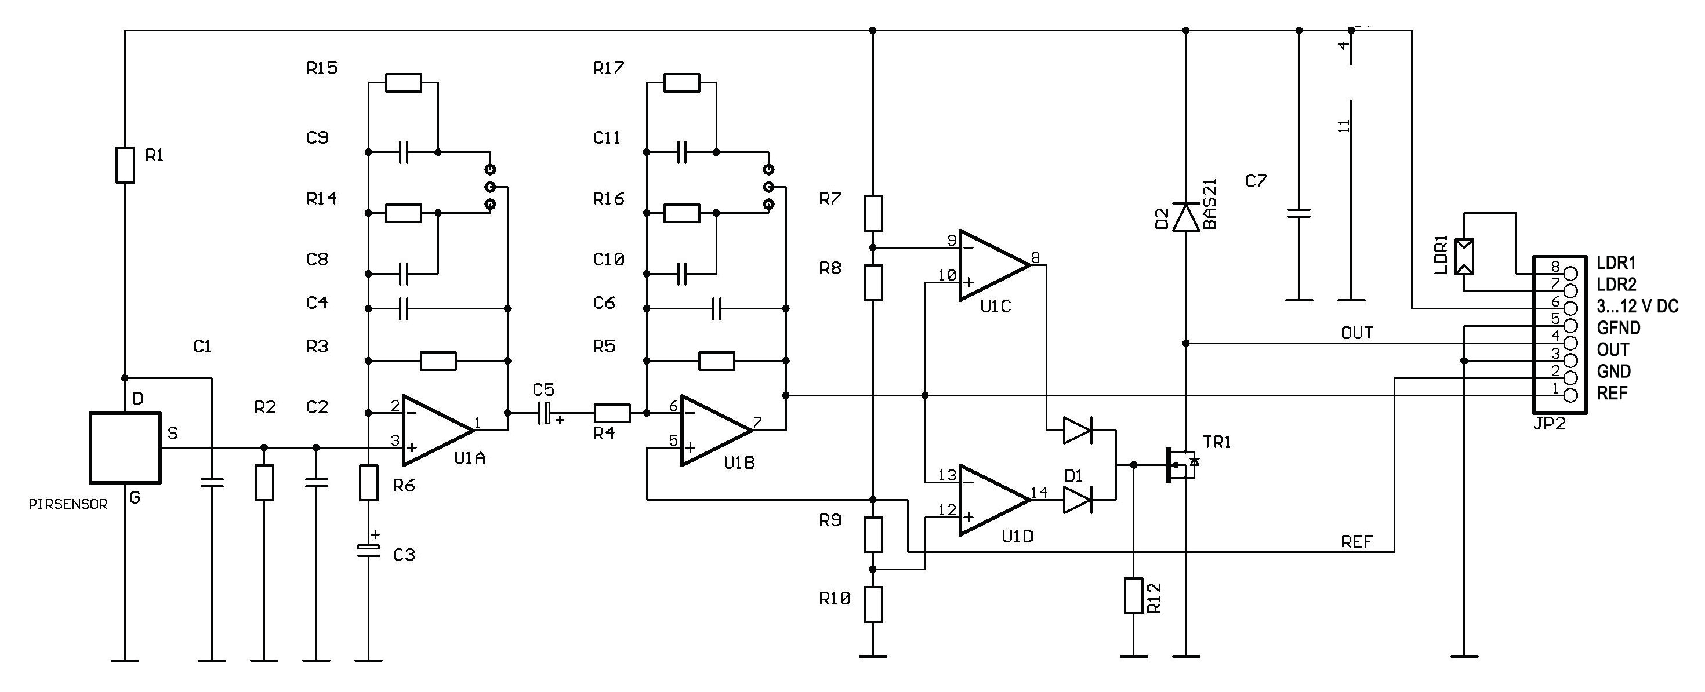
\includegraphics[width=0.75\textwidth]{img/pirstd.png}
\caption{Scheme of PIR STD.\cite{PIROperationalManual}\label{fig:pirstdscheme}}
\end{center}
\end{figure}

\paragraph{I. stage}
The first one starts at S of the PIR sensor, following with noise/lowpass filter consisting
of the amplifier $U1A$ and the feedback components $R3$, $C4$, $C8$, $R14$, $C9$, $R14$.
There is also highpass filter done by $R6$ and $C3$. The output of this stage is a signal
with frequency between $f_{L1}$ and $f_{H1}$ amplified $A_{U1A}$ times.

\begin{subequations}
\begin{equation}
f_{H1} = \frac{1}{2 \pi R_{3,14} C_{4,8}}
\end{equation}

\begin{equation}
f_{H1}^{'} = \frac{1}{2 \pi R_{3,15} C_{4,9}}
\end{equation}
\end{subequations}

The choice of resistor $R_{3,14} / R_{3,15}$ and capacitator $C_{4,8} / C_{4,9}$
is done by connected switch. The value of resistance and capacitance of the
components can be counted with formula for parallel connection.

\begin{equation}
R_{A,B}^{p} = \frac{1}{R_A} + \frac{1}{R_B}
\end{equation}

\begin{equation}
C_{A,B}^{p} = C_A + C_B
\end{equation}

The same for the resistors $R_{5,16}$ and $R_{5,17}$ and capacitators $C_{6,10}$ and $C_{6,11}$.

\begin{equation}
f_{L1} = \frac{1}{2 \pi R_6 C_3}
\end{equation}

\begin{subequations}
\begin{equation}
A_{U1A} = 1 + \frac{R_{3,14}}{R_2}
\end{equation}
\begin{equation}
A_{U1A} = 1 + \frac{R_{3,15}}{R_2}
\end{equation}
\end{subequations}

\paragraph{II. stage}
The second processing stage focuses on amplification. It also includes lowpass filtering done
by $C5$ and $R4$ and highpass filter performed by the feedback of amplifier $U1B$. The greater
amplification is also made by the divider bridge ($R8$, $R9$, $R10$, $R11$) connected to the
positive input. The output of frequency between $max(f_{L1}, f_{L2})$ and $min(f_{H1}, f_{H2})$
amplified $A_{U1A} \cdot A_{U1B}$ times is an analog output connected to the pin 1.

\begin{equation}
f_{H2} = \frac{1}{2 \pi R_5 C_6}
\end{equation}

\begin{equation}
f_{L2} = \frac{1}{2 \pi R_4 C_5}
\end{equation}

\begin{equation}
A_{U1B} = -\frac{R_5}{R_4}
\end{equation}

\paragraph{III. stage}
The third phase performs top-bottom tresholding generating binary output
used in simple industrial application. It is not used in the project.\cite{PIRSchemeDescription}


\subsection*{Connecting the sensor}
PIR sensor is connected to the MCU. Except for source, ground and output which are connected directly,
{\it PIR STD} has also reference voltage input, that should be approximately $\frac{V_cc}{2}~V$.
To ensure that a voltage divider is used with two resistors of the same resistance $R_X$.
During the testing $100~k\Omega$ resistors were used. The circuit is shown in the figure \ref{fig:PIRcircuit}.

\begin{figure}[h!]
\begin{center}
\begin{circuitikz}
\ctikzset{bipoles/generic/height=0.2}
\ctikzset { label/align = straight }
\draw %(2,0)

  %to[V=$V_{Th}$] (0,2)
  %to[R=$R_{Th}$] (2.5,2)
  %to[short,i=$I$, -o] (4,2)
  %to[short] (4.5,2)
  % ref
  (0,2) to[short, l={\tiny $REF$}, o-]
  (1,2) to[short]
  (4,2) to[R={\tiny $R_{X}$}]
  (6,2) to[short,-*] (6,1.5)

  (2,0.5) to[short,*-]
  (2,2.5) to[R={\tiny $R_{X}$}]
  (4,2.5) to[short,-*] (4,2) 
  
  
  
  % vcc
  (0,1.5) to[short, l={\tiny $VCC$}, o-]
  (1,1.5) to[short]
  (7,1.5) to[short, l={\tiny $5~V$}, -o] (8,1.5)
  % signal
  (0,1) to[short, l={\tiny $ANA$}, o-] 
  (1,1) to[short]
  (7,1) to[short, l={\tiny $A1$}, -o] (8,1)
  % gnd
  (0,0.5) to[short, l={\tiny $GND$}, o-]
  (1,0.5) to[short]
  (7,0.5) to[short, l={\tiny $GND$}, -o] (8,0.5)

;
\node[draw,minimum width=2.5cm,minimum height=2.5cm,anchor=south east] at (0,0){PIR};
\node[draw,minimum width=2.5cm,minimum height=2.5cm,anchor=south west] at (8,0){MCU};
\end{circuitikz}
\caption{Connection of PIR and MCU.\label{fig:PIRcircuit}}
\end{center}
\end{figure}


\subsection*{Sampling}
The module is programmed to read signal in sampling frequency and send the data to server.

\paragraph{AD conversion}
The projection of voltage to a value is done by the built-in functionality, accessible by
standard library function \texttt{analogRead()}. The sets of analog values $A$ and digital values $D$
according to documentation of the function\cite{ArduinoAnalogRead} and the sensor\cite{PIROperationalManual}
and the morphism $c$ are shown in the formula \ref{eq:ad_projection}.

\begin{subequations}
\begin{equation}
A = \langle 0;V_{cc}\rangle
\end{equation}
\begin{equation}
D = \{0; 1; ..., 1023\}
\end{equation}
\begin{equation}
c: A \rightarrow D = x_A \rightarrow \frac{1023x_A}{V_{cc}}, x_A \in D
\end{equation}
\label{eq:ad_projection}
\end{subequations}

\paragraph{Sampling frequency}
The usable sampling frequency can be estimated: the fresnel lens of {\it PIR STD} splits the
area into $10^{\circ}$ circular sectors. Object moving around the sensor in the distance $0.5~m$
with speed $15~km.h^{-1} = 4.1667~m.s^{-1}$ (very fast run) passes the central circular sector in

\begin{equation}
t = \frac{s}{v} = \frac{0.5*tg(10^{\circ})}{4.1667} = 0.02116~s
\end{equation}

This means the frequency of the movement through the circular sectors is

\begin{equation}
f = \frac{1}{t} = \frac{1}{0.02116} = 47.259~Hz
\end{equation}

According to Shannon theorem\cite{DigitalSignalProcessing}, the sampling frequency must be at least twice as big as the
maximal frequency in the signal, which leads to

\begin{equation}
Fs \geq 2*47.259 = 94.518 
\end{equation}

Rounding up gives us minimal sampling frequency $100~Hz$, or sampling period $10~ms$.
resulting with $2B$ sample in throughput $\mu$

\begin{equation}
\mu = F_s * |\text{sample}| * 8\frac{bit}{byte} = 100 * 2 * 8 = 1.6~kbps
\end{equation}


\subsection*{MCU Program}
The MCU is programmed to sample data with fixed sampling frequency and form the sequential
segments out of it. A $N$-sized segment is then sent away using ESP8266 present at the module.
A multicast technology is used, enabling multiple servers to work over the data concurrently
and also ease of initialization of communication, where the channel is predefined, so
no mutual IP address is needed. The sending frequency can be derived from sampling frequency $F_s$
with formula \ref{eq:sendfrequency}.

\begin{equation}
F_{send} = \frac{F_s}{N}
\label{eq:sendfrequency}
\end{equation}

MCU runs a HTTP server, enabling the MCU to be configured remotely. It is possible to set
sampling frequency or period with the altering other correspondingly as same as sending period,
frequency, or segment size with a maximal segment size \textbf{here will be MAXSEGMENTSIZE}.
The REST API also enables to set the multicast channel, both address and port, turning
debugging informations on/off to serial line.

The complete REST API description is to be seen in the appendix \ref{appendix:mcu_restapi}.




\section{Classification server}
{\it Monitor} is the classification server, that collects data from the sensors and performs
classification algorithms described in \ref{section:classification} with it. {\it Finish}

\subsection*{Data sources}
Monitor enables reading data from serial port, multicast channel and replaying saved data from file.
This feature is done using class \texttt{Reader} from the module \texttt{comm} and inherited classes
in modules \texttt{comm\_serial}, \texttt{comm\_mcast}, \texttt{comm\_replay}.

Class Reader corresponds with the design pattern Singleton, holding one single instance for each
serial port, multicast channel and file to avoid opening multiple handles and potential data race.

Instantiation of the object is done in the first demand for it in the call of static method \texttt{getReader()}.
Each object then possess separate reading thread, that ensures updating of the data. Getting the last
received segment is through method \texttt{getSegment()}, a thread lock is used. The whole design is shown
in the figure \ref{fig:class_src}.

\begin{figure}[h!]
\begin{center}
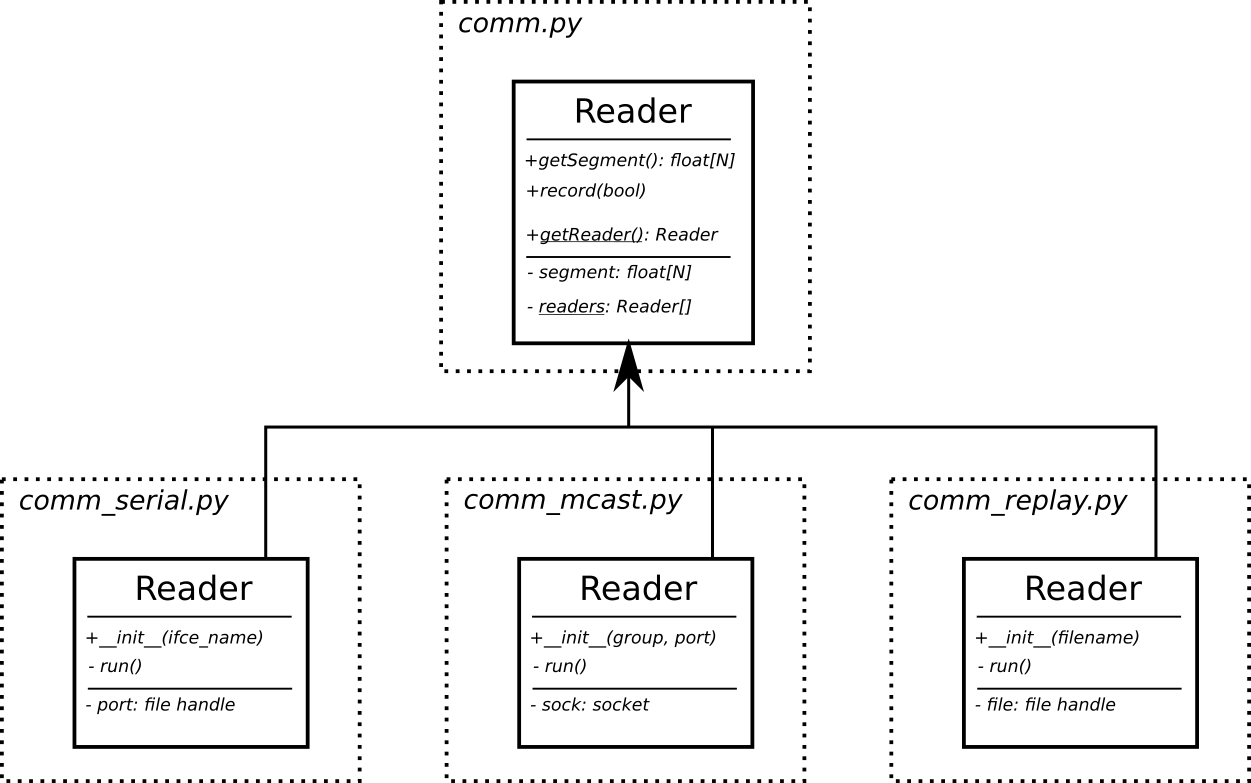
\includegraphics[width=0.8\textwidth]{img/class_src.png}
\caption{UML diagram of Reader classes. \label{fig:class_src}}
\end{center}
\end{figure}

{\it ...}

\subsection*{Classification}
The segmentation 
{\it Implementation of linear regression.}







%\section{Collector} 
%{\it Collector} is a program, as the name says, that collects data from sensors and implements
%the whole described algorithm. Classified objects are then sent to a {\it visualizer}.

%\subsection*{Communication}
%The communication of the sensor module and the client app is designed as a client-server. The results
%from the classification performed by server are sent to the client which shows it to user.

%As the technology for the channel a LAN multicast stream is used at 224.0.0.128:12345.
%The main advantage in comparison to unicast is a support of multiple clients.

%\section{Visualizer}
%Client app called {\it Visualizer} is written in {\it Python3} and graphical library {\it Tkinter}.
%This choice was made with portability of the program taken into consideration.
%The design of user interface is described in chapter \ref{Label:UI}.




\chapter{Experiments}

\section{Evaluation}
A several metrics can be used to evaluate the success rate of decision.
In following equations, $A$ stands for tuple of $|A|$ artefacts being
evaluated, $A[i]$ for an artefact from this set. For each artefact from testing
set, a label $\kappa_{A[i]^{X}}$ for all traits is known.

For labeling purposes, a variation of Lukasiewicz logic was used to cover
the states, which Bool logic is not able to handle, as the position of person
in case area is empty. The operation in the table \ref{table:3stateLogicOp} is
represents comparing the computed score and the real label returning a score
of success of the decision.

Input conditions for fuzzy number $a \in \in \langle 0;1 \rangle$
and $\kappa \in \{ 1, 0, N\}$, which is in {\it json} file format represented
by {\it True}, {\it False} and {\it None} literals respectively. The output
is a success rate, multiplied by $100$ can be converted to percentage.

\begin{table}
\begin{center}
\begin{tabular}{|c|c|c|} \hline
\textbf{a}  & \textbf{$\kappa$} & \textbf{$a \cdot \kappa$} \\ \hline
$a$         & 1               & $a$                       \\ \hline
$a$         & 0               & $N(a)$                    \\ \hline
$a$         & N               & \it{excluded}             \\ \hline
\end{tabular}
\caption{Classifier output comparing to reference.\label{table:3stateLogicOp} }
\end{center}
\end{table}

To emulate the decision by tresholding a fuzzy sigmoid can be applied to $a$,
mapping fuzzy values to fuzzy values, which are more decisive. An example is
shown at the equation \ref{eq:fuzzySigmoid}. The usage and choice of such
function distorts results significantly.

\begin{equation}
\sigma(a) = \begin{cases} 1 & a \geq 0.5 \\
            0 & \text{otherwise} \end{cases}
\label{eq:fuzzySigmoid}
\end{equation}

The metrics used and described below use also notation described by the equations
\ref{eq:tupleArtefactNotation}. These tuples contains only artefacts, that are
positive for the trait $X$ ($A_{X}^{1}$), or negative ($A_{X}^{0}$).

\begin{subequations}
\begin{equation}
A_{X}^{1} = (\forall a \in A: \kappa_{X}(a) = 1)
\end{equation}
\begin{equation}
A_{X}^{0} = (\forall a \in A \kappa_{X}(a) = 0)
\end{equation}
\label{eq:tupleArtefactNotation}
\end{subequations}

First possible metric is a simple average of artefacts with its scores by the
formula \ref{eq:artefactAverage} for trait $X$. Similarly can be counted
separately success rate for $A_{X}^{1}$ and $A_{X}^{0}$.

\begin{equation}
\overline{A_{X}} = \frac{1}{|A|} \sum_{a\in A} a_{X} \cdot \kappa_{X}(a)
\label{eq:artefactAverage}
\end{equation}

The metric \ref{eq:artefactAverage} does not take account of artefact length
as a weight. To do so, the formula is altered with a weight added at the
formula \ref{eq:artefactWeightedAverage}.

\begin{equation}
\overline{A_{X}} = \sum_{a\in A} (a_{X} \cdot \kappa_{X}(a))\frac{|a|}{\sum_{A}|a|}
\label{eq:artefactWeightedAverage}
\end{equation}

Unit tests were created to verify the program components. It uses {\it Boost.Test},
framework for creating unit tests which is part of {\it C++ Boost} library set.
The testing program placed in folder {\it collector/tests/} is linked with
{\it collector} transformed in static library.

{\it
Metodika a vysledky. Muze zahrnovat i matematicke dukazu, postupy...

Interpretace vysledku a moznosti nasazeni v praxi.

HW narocnost -- CPU, pamet, chovani pri paralelizaci apod.
}




\chapter{User Interface}
\label{Label:UI}

{\it Description of visualizer}

\begin{figure}[h!]
\begin{center}
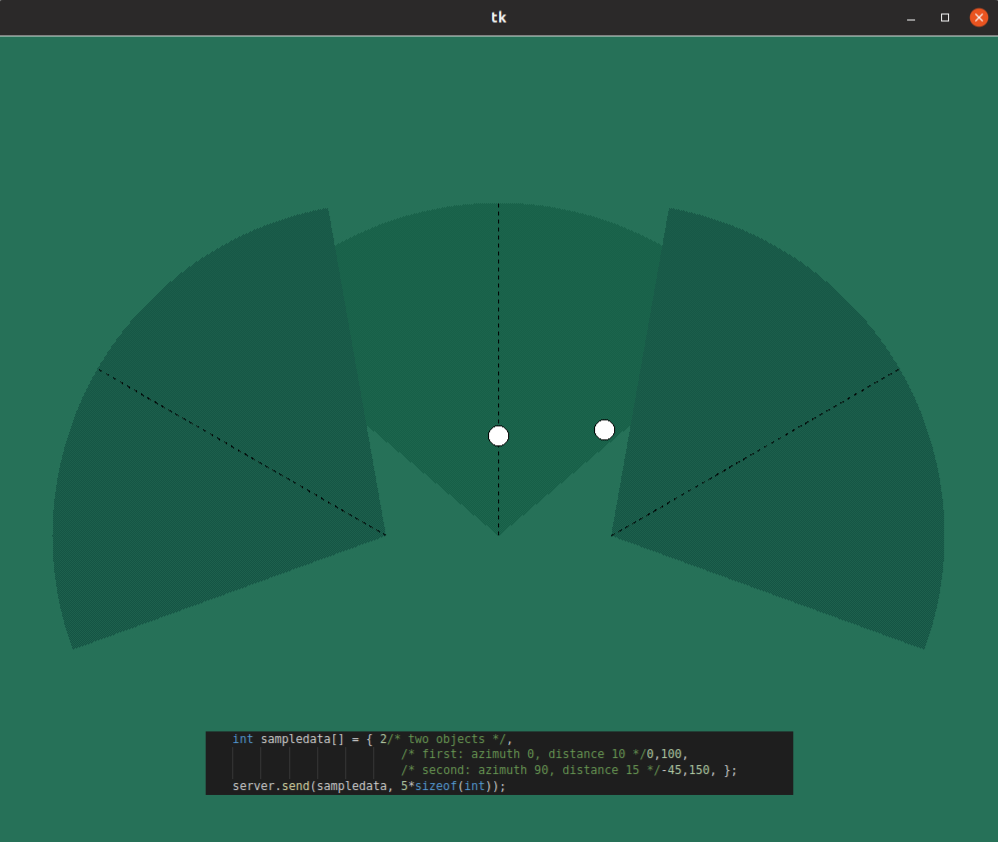
\includegraphics[width=0.6\textwidth]{img/visualizer.png}
\caption{Visualizer prototype with sample data. {\it Will be replaced.} \label{fig:visualizer}}
\end{center}
\end{figure}






\chapter{Conclusion}
Shrnuti zameru prace. Zhodnoceni splneni (i formalnich bodu).

Zhodnoceni z pohledu dalsiho vyvoje. Co se nestihlo (a dalo by se jeste).

Bez odkazu do textu / literatury. Zadne nove poznatky, cisla a grafy.

Pekny postreh k praci (co jsem se naucil).

Vyhled do budoucna, rozdeleni na casti.

20 stranek SEP, 40 bakalarka.




%===============================================================================
